% Options for packages loaded elsewhere
% Options for packages loaded elsewhere
\PassOptionsToPackage{unicode}{hyperref}
\PassOptionsToPackage{hyphens}{url}
\PassOptionsToPackage{dvipsnames,svgnames,x11names}{xcolor}
%
\documentclass[
  letterpaper,
  DIV=11,
  numbers=noendperiod]{scrreprt}
\usepackage{xcolor}
\usepackage{amsmath,amssymb}
\setcounter{secnumdepth}{2}
\usepackage{iftex}
\ifPDFTeX
  \usepackage[T1]{fontenc}
  \usepackage[utf8]{inputenc}
  \usepackage{textcomp} % provide euro and other symbols
\else % if luatex or xetex
  \usepackage{unicode-math} % this also loads fontspec
  \defaultfontfeatures{Scale=MatchLowercase}
  \defaultfontfeatures[\rmfamily]{Ligatures=TeX,Scale=1}
\fi
\usepackage{lmodern}
\ifPDFTeX\else
  % xetex/luatex font selection
\fi
% Use upquote if available, for straight quotes in verbatim environments
\IfFileExists{upquote.sty}{\usepackage{upquote}}{}
\IfFileExists{microtype.sty}{% use microtype if available
  \usepackage[]{microtype}
  \UseMicrotypeSet[protrusion]{basicmath} % disable protrusion for tt fonts
}{}
\makeatletter
\@ifundefined{KOMAClassName}{% if non-KOMA class
  \IfFileExists{parskip.sty}{%
    \usepackage{parskip}
  }{% else
    \setlength{\parindent}{0pt}
    \setlength{\parskip}{6pt plus 2pt minus 1pt}}
}{% if KOMA class
  \KOMAoptions{parskip=half}}
\makeatother
% Make \paragraph and \subparagraph free-standing
\makeatletter
\ifx\paragraph\undefined\else
  \let\oldparagraph\paragraph
  \renewcommand{\paragraph}{
    \@ifstar
      \xxxParagraphStar
      \xxxParagraphNoStar
  }
  \newcommand{\xxxParagraphStar}[1]{\oldparagraph*{#1}\mbox{}}
  \newcommand{\xxxParagraphNoStar}[1]{\oldparagraph{#1}\mbox{}}
\fi
\ifx\subparagraph\undefined\else
  \let\oldsubparagraph\subparagraph
  \renewcommand{\subparagraph}{
    \@ifstar
      \xxxSubParagraphStar
      \xxxSubParagraphNoStar
  }
  \newcommand{\xxxSubParagraphStar}[1]{\oldsubparagraph*{#1}\mbox{}}
  \newcommand{\xxxSubParagraphNoStar}[1]{\oldsubparagraph{#1}\mbox{}}
\fi
\makeatother

\usepackage{color}
\usepackage{fancyvrb}
\newcommand{\VerbBar}{|}
\newcommand{\VERB}{\Verb[commandchars=\\\{\}]}
\DefineVerbatimEnvironment{Highlighting}{Verbatim}{commandchars=\\\{\}}
% Add ',fontsize=\small' for more characters per line
\usepackage{framed}
\definecolor{shadecolor}{RGB}{241,243,245}
\newenvironment{Shaded}{\begin{snugshade}}{\end{snugshade}}
\newcommand{\AlertTok}[1]{\textcolor[rgb]{0.68,0.00,0.00}{#1}}
\newcommand{\AnnotationTok}[1]{\textcolor[rgb]{0.37,0.37,0.37}{#1}}
\newcommand{\AttributeTok}[1]{\textcolor[rgb]{0.40,0.45,0.13}{#1}}
\newcommand{\BaseNTok}[1]{\textcolor[rgb]{0.68,0.00,0.00}{#1}}
\newcommand{\BuiltInTok}[1]{\textcolor[rgb]{0.00,0.23,0.31}{#1}}
\newcommand{\CharTok}[1]{\textcolor[rgb]{0.13,0.47,0.30}{#1}}
\newcommand{\CommentTok}[1]{\textcolor[rgb]{0.37,0.37,0.37}{#1}}
\newcommand{\CommentVarTok}[1]{\textcolor[rgb]{0.37,0.37,0.37}{\textit{#1}}}
\newcommand{\ConstantTok}[1]{\textcolor[rgb]{0.56,0.35,0.01}{#1}}
\newcommand{\ControlFlowTok}[1]{\textcolor[rgb]{0.00,0.23,0.31}{\textbf{#1}}}
\newcommand{\DataTypeTok}[1]{\textcolor[rgb]{0.68,0.00,0.00}{#1}}
\newcommand{\DecValTok}[1]{\textcolor[rgb]{0.68,0.00,0.00}{#1}}
\newcommand{\DocumentationTok}[1]{\textcolor[rgb]{0.37,0.37,0.37}{\textit{#1}}}
\newcommand{\ErrorTok}[1]{\textcolor[rgb]{0.68,0.00,0.00}{#1}}
\newcommand{\ExtensionTok}[1]{\textcolor[rgb]{0.00,0.23,0.31}{#1}}
\newcommand{\FloatTok}[1]{\textcolor[rgb]{0.68,0.00,0.00}{#1}}
\newcommand{\FunctionTok}[1]{\textcolor[rgb]{0.28,0.35,0.67}{#1}}
\newcommand{\ImportTok}[1]{\textcolor[rgb]{0.00,0.46,0.62}{#1}}
\newcommand{\InformationTok}[1]{\textcolor[rgb]{0.37,0.37,0.37}{#1}}
\newcommand{\KeywordTok}[1]{\textcolor[rgb]{0.00,0.23,0.31}{\textbf{#1}}}
\newcommand{\NormalTok}[1]{\textcolor[rgb]{0.00,0.23,0.31}{#1}}
\newcommand{\OperatorTok}[1]{\textcolor[rgb]{0.37,0.37,0.37}{#1}}
\newcommand{\OtherTok}[1]{\textcolor[rgb]{0.00,0.23,0.31}{#1}}
\newcommand{\PreprocessorTok}[1]{\textcolor[rgb]{0.68,0.00,0.00}{#1}}
\newcommand{\RegionMarkerTok}[1]{\textcolor[rgb]{0.00,0.23,0.31}{#1}}
\newcommand{\SpecialCharTok}[1]{\textcolor[rgb]{0.37,0.37,0.37}{#1}}
\newcommand{\SpecialStringTok}[1]{\textcolor[rgb]{0.13,0.47,0.30}{#1}}
\newcommand{\StringTok}[1]{\textcolor[rgb]{0.13,0.47,0.30}{#1}}
\newcommand{\VariableTok}[1]{\textcolor[rgb]{0.07,0.07,0.07}{#1}}
\newcommand{\VerbatimStringTok}[1]{\textcolor[rgb]{0.13,0.47,0.30}{#1}}
\newcommand{\WarningTok}[1]{\textcolor[rgb]{0.37,0.37,0.37}{\textit{#1}}}

\usepackage{longtable,booktabs,array}
\usepackage{calc} % for calculating minipage widths
% Correct order of tables after \paragraph or \subparagraph
\usepackage{etoolbox}
\makeatletter
\patchcmd\longtable{\par}{\if@noskipsec\mbox{}\fi\par}{}{}
\makeatother
% Allow footnotes in longtable head/foot
\IfFileExists{footnotehyper.sty}{\usepackage{footnotehyper}}{\usepackage{footnote}}
\makesavenoteenv{longtable}
\usepackage{graphicx}
\makeatletter
\newsavebox\pandoc@box
\newcommand*\pandocbounded[1]{% scales image to fit in text height/width
  \sbox\pandoc@box{#1}%
  \Gscale@div\@tempa{\textheight}{\dimexpr\ht\pandoc@box+\dp\pandoc@box\relax}%
  \Gscale@div\@tempb{\linewidth}{\wd\pandoc@box}%
  \ifdim\@tempb\p@<\@tempa\p@\let\@tempa\@tempb\fi% select the smaller of both
  \ifdim\@tempa\p@<\p@\scalebox{\@tempa}{\usebox\pandoc@box}%
  \else\usebox{\pandoc@box}%
  \fi%
}
% Set default figure placement to htbp
\def\fps@figure{htbp}
\makeatother


% definitions for citeproc citations
\NewDocumentCommand\citeproctext{}{}
\NewDocumentCommand\citeproc{mm}{%
  \begingroup\def\citeproctext{#2}\cite{#1}\endgroup}
\makeatletter
 % allow citations to break across lines
 \let\@cite@ofmt\@firstofone
 % avoid brackets around text for \cite:
 \def\@biblabel#1{}
 \def\@cite#1#2{{#1\if@tempswa , #2\fi}}
\makeatother
\newlength{\cslhangindent}
\setlength{\cslhangindent}{1.5em}
\newlength{\csllabelwidth}
\setlength{\csllabelwidth}{3em}
\newenvironment{CSLReferences}[2] % #1 hanging-indent, #2 entry-spacing
 {\begin{list}{}{%
  \setlength{\itemindent}{0pt}
  \setlength{\leftmargin}{0pt}
  \setlength{\parsep}{0pt}
  % turn on hanging indent if param 1 is 1
  \ifodd #1
   \setlength{\leftmargin}{\cslhangindent}
   \setlength{\itemindent}{-1\cslhangindent}
  \fi
  % set entry spacing
  \setlength{\itemsep}{#2\baselineskip}}}
 {\end{list}}
\usepackage{calc}
\newcommand{\CSLBlock}[1]{\hfill\break\parbox[t]{\linewidth}{\strut\ignorespaces#1\strut}}
\newcommand{\CSLLeftMargin}[1]{\parbox[t]{\csllabelwidth}{\strut#1\strut}}
\newcommand{\CSLRightInline}[1]{\parbox[t]{\linewidth - \csllabelwidth}{\strut#1\strut}}
\newcommand{\CSLIndent}[1]{\hspace{\cslhangindent}#1}



\setlength{\emergencystretch}{3em} % prevent overfull lines

\providecommand{\tightlist}{%
  \setlength{\itemsep}{0pt}\setlength{\parskip}{0pt}}



 


\KOMAoption{captions}{tableheading}
\makeatletter
\@ifpackageloaded{tcolorbox}{}{\usepackage[skins,breakable]{tcolorbox}}
\@ifpackageloaded{fontawesome5}{}{\usepackage{fontawesome5}}
\definecolor{quarto-callout-color}{HTML}{909090}
\definecolor{quarto-callout-note-color}{HTML}{0758E5}
\definecolor{quarto-callout-important-color}{HTML}{CC1914}
\definecolor{quarto-callout-warning-color}{HTML}{EB9113}
\definecolor{quarto-callout-tip-color}{HTML}{00A047}
\definecolor{quarto-callout-caution-color}{HTML}{FC5300}
\definecolor{quarto-callout-color-frame}{HTML}{acacac}
\definecolor{quarto-callout-note-color-frame}{HTML}{4582ec}
\definecolor{quarto-callout-important-color-frame}{HTML}{d9534f}
\definecolor{quarto-callout-warning-color-frame}{HTML}{f0ad4e}
\definecolor{quarto-callout-tip-color-frame}{HTML}{02b875}
\definecolor{quarto-callout-caution-color-frame}{HTML}{fd7e14}
\makeatother
\makeatletter
\@ifpackageloaded{bookmark}{}{\usepackage{bookmark}}
\makeatother
\makeatletter
\@ifpackageloaded{caption}{}{\usepackage{caption}}
\AtBeginDocument{%
\ifdefined\contentsname
  \renewcommand*\contentsname{Table of contents}
\else
  \newcommand\contentsname{Table of contents}
\fi
\ifdefined\listfigurename
  \renewcommand*\listfigurename{List of Figures}
\else
  \newcommand\listfigurename{List of Figures}
\fi
\ifdefined\listtablename
  \renewcommand*\listtablename{List of Tables}
\else
  \newcommand\listtablename{List of Tables}
\fi
\ifdefined\figurename
  \renewcommand*\figurename{Figure}
\else
  \newcommand\figurename{Figure}
\fi
\ifdefined\tablename
  \renewcommand*\tablename{Table}
\else
  \newcommand\tablename{Table}
\fi
}
\@ifpackageloaded{float}{}{\usepackage{float}}
\floatstyle{ruled}
\@ifundefined{c@chapter}{\newfloat{codelisting}{h}{lop}}{\newfloat{codelisting}{h}{lop}[chapter]}
\floatname{codelisting}{Listing}
\newcommand*\listoflistings{\listof{codelisting}{List of Listings}}
\makeatother
\makeatletter
\makeatother
\makeatletter
\@ifpackageloaded{caption}{}{\usepackage{caption}}
\@ifpackageloaded{subcaption}{}{\usepackage{subcaption}}
\makeatother
\usepackage{bookmark}
\IfFileExists{xurl.sty}{\usepackage{xurl}}{} % add URL line breaks if available
\urlstyle{same}
\hypersetup{
  pdftitle={PAD},
  pdfauthor={Tom Baladrón},
  colorlinks=true,
  linkcolor={blue},
  filecolor={Maroon},
  citecolor={Blue},
  urlcolor={Blue},
  pdfcreator={LaTeX via pandoc}}


\title{PAD}
\usepackage{etoolbox}
\makeatletter
\providecommand{\subtitle}[1]{% add subtitle to \maketitle
  \apptocmd{\@title}{\par {\large #1 \par}}{}{}
}
\makeatother
\subtitle{Unidad de Psicometría y Análisis de Datos - Mide UC}
\author{Tom Baladrón}
\date{2025-07-17}
\begin{document}
\maketitle

\renewcommand*\contentsname{Table of contents}
{
\hypersetup{linkcolor=}
\setcounter{tocdepth}{2}
\tableofcontents
}

\bookmarksetup{startatroot}

\chapter*{Preface}\label{preface}
\addcontentsline{toc}{chapter}{Preface}

\markboth{Preface}{Preface}

This is a Quarto book.

To learn more about Quarto books visit
\url{https://quarto.org/docs/books}.

{[}1{]} 2

\bookmarksetup{startatroot}

\chapter*{Sobre el autor}\label{sobre-el-autor}
\addcontentsline{toc}{chapter}{Sobre el autor}

\markboth{Sobre el autor}{Sobre el autor}

This is a book created from markdown and executable code.

See Knuth (1984) for additional discussion of literate programming.

{[}1{]} 2

\bookmarksetup{startatroot}

\chapter*{Agradecimientos}\label{agradecimientos}
\addcontentsline{toc}{chapter}{Agradecimientos}

\markboth{Agradecimientos}{Agradecimientos}

In summary, this book has no content whatsoever.

{[}1{]} 2

\part{Módulo teórico}

\chapter{Recuerdo matemático}\label{recuerdo-matemuxe1tico}

\section{MEDIDAS DE TENDENCIA
CENTRAL}\label{medidas-de-tendencia-central}

\subsection{Media}\label{media}

La \textbf{media} se obtiene sumando todos los valores de un conjunto de
datos y dividiendo esta suma entre el número total de valores.

\[
Media: \bar{x} = \frac{\sum_{i=1}^{n} x_i}{n}
\]

Donde:

\begin{itemize}
\item
  \(\bar{x}\) = promedio.
\item
  \(x_i\) = puntaje del elemento i.
\item
  \(n\) = cantidad total de elementos.
\end{itemize}

\subsection{Mediana}\label{mediana}

La \textbf{mediana} es el valor que se encuentra en el medio de un
conjunto de datos ordenados. Si el número de datos es impar, la mediana
es el valor central. Si es par, la mediana es el promedio de los dos
valores centrales. La mediana es útil porque no se ve afectada por
valores atípicos.

\[
Mediana:\begin{cases} 
\tilde{x} = x_{(\frac{n+1}{2})} & \text{si } n \text{ es impar} \\ 
\tilde{x} = \frac{x_{(\frac{n}{2})} \ + \ x_{(\frac{n}{2} + 1)}}{2} & \text{si } n \text{ es par} 
\end{cases}
\]

Donde:

\begin{itemize}
\tightlist
\item
  \(\tilde{x}\) = mediana.
\item
  \(n\) = cantidad total de elementos.
\item
  \(()\) = implica buscar el elemento en la posición señalada dentro del
  paréntesis.
\end{itemize}

\subsection{Moda}\label{moda}

La \textbf{moda} es el valor o valores que aparecen con mayor frecuencia
en un conjunto de datos.

\[
\text{Moda: } x_{\text{moda}} = \{x_i: \text{frecuencia}(x_i) \text{ es máxima}\}
\]

Donde:

\begin{itemize}
\tightlist
\item
  \(X_{\text{moda}}\) = moda.
\item
  \(\text{{}}\) = símbolo para una condición que se debe cumplir.
\end{itemize}

\section{MEDIDAS DE DISPERSIÓN}\label{medidas-de-dispersiuxf3n}

\subsection{Rango}\label{rango}

El \textbf{rango} mide la diferencia entre el valor máximo y el valor
mínimo en un conjunto de datos. Es una medida simple de la dispersión.

\[
\text{Rango} = x_{\text{max}} - x_{\text{min}}
\]

Donde:

\begin{itemize}
\tightlist
\item
  \(x_{\text{max}}\) = valor máximo.
\item
  \(x_{\text{min}}\) = valor mínimo.
\end{itemize}

\subsection{Rango inter-cuartil}\label{rango-inter-cuartil}

El \textbf{rango inter-cuartil} (\textbf{IQR}) mide la dispersión de los
datos en el rango entre el primer cuartil (Q1) y el tercer cuartil (Q3).
Es útil para identificar la dispersión sin ser afectado por valores
extremos.

\[
\text{IQR} = Q_{3} - Q_{1}
\]

Donde:

\begin{itemize}
\tightlist
\item
  \(Q_{1}\) = primer cuartil (25\% de los datos están por debajo).
\item
  \(Q_{3}\) = tercer cuartil (75\% de los datos están por debajo).
\end{itemize}

\subsection{Suma de cuadrados}\label{suma-de-cuadrados}

La \textbf{suma de cuadrados} (\textbf{SS}) es una medida que calcula la
suma de las diferencias al cuadrado entre cada valor y la media. Es un
componente esencial para calcular la varianza y la desviación estándar.

\[
\text{SS} = \sum_{i=1}^{n} (x_i - \bar{x})^2
\]

Donde:

\begin{itemize}
\tightlist
\item
  \(x_i\) = valores de los datos.
\item
  \(\bar{x}\) = media de los datos.
\end{itemize}

\subsection{Varianza}\label{varianza}

La \textbf{varianza} (\textbf{σ2}) mide la dispersión o variabilidad de
un conjunto de datos respecto a su media. Indica cuánto se desvían los
datos individuales de la media en promedio.

\begin{longtable}[]{@{}
  >{\raggedright\arraybackslash}p{(\linewidth - 2\tabcolsep) * \real{0.5657}}
  >{\raggedright\arraybackslash}p{(\linewidth - 2\tabcolsep) * \real{0.4343}}@{}}
\toprule\noalign{}
\begin{minipage}[b]{\linewidth}\raggedright
En función del promedio (\(\bar{x}\)) :
\end{minipage} & \begin{minipage}[b]{\linewidth}\raggedright
En función de la suma de cuadrados (SS):
\end{minipage} \\
\midrule\noalign{}
\endhead
\bottomrule\noalign{}
\endlastfoot
\(
\sigma^2 = \frac{\sum_{i=1}^{n} (x_i - \bar{x})^2}{n}
\) & \(
\sigma^2 = \frac{\text{SS}}{n}
\) \\
\begin{minipage}[t]{\linewidth}\raggedright
Donde:

\begin{itemize}
\tightlist
\item
  \(\sigma^2\) = varianza.
\item
  \(x_i\) = valores de los datos.
\item
  \(\bar{x}\) = media de los datos.
\item
  \(n\) = número total de elementos.
\end{itemize}
\end{minipage} & \begin{minipage}[t]{\linewidth}\raggedright
Donde:

\begin{itemize}
\tightlist
\item
  \(\text{SS}\) = suma de cuadrados.
\item
  \(n\) = número total de elementos.
\end{itemize}
\end{minipage} \\
\end{longtable}

\textbf{Caso especial} de varianza para \textbf{variables dicotómicas}
donde se puede conceptualizar uno de los valores como ``acierto'' y el
otro como ``fracaso''.

\[
\sigma^2 = p(1-p)
\]

Donde:

\begin{itemize}
\tightlist
\item
  \(\sigma^2\) = varianza.
\item
  \(p\) = probabilidad de éxito (ej. proporción de respuestas
  correctas).
\end{itemize}

\subsection{Desviación estándar}\label{desviaciuxf3n-estuxe1ndar}

La \textbf{desviación estándar} ( \(\sigma\) ) es la raíz cuadrada de la
varianza. Proporciona una medida de dispersión que está en las mismas
unidades que los datos originales, facilitando la interpretación.

\begin{longtable}[]{@{}
  >{\raggedright\arraybackslash}p{(\linewidth - 4\tabcolsep) * \real{0.4388}}
  >{\raggedright\arraybackslash}p{(\linewidth - 4\tabcolsep) * \real{0.2734}}
  >{\raggedright\arraybackslash}p{(\linewidth - 4\tabcolsep) * \real{0.2806}}@{}}
\toprule\noalign{}
\begin{minipage}[b]{\linewidth}\raggedright
En f(x) del promedio
\end{minipage} & \begin{minipage}[b]{\linewidth}\raggedright
En f(x) de la varianza
\end{minipage} & \begin{minipage}[b]{\linewidth}\raggedright
En f(x) de la suma de cuadrados
\end{minipage} \\
\midrule\noalign{}
\endhead
\bottomrule\noalign{}
\endlastfoot
\(
\sigma = \sqrt{\frac{\sum_{i=1}^{n} (x_i - \bar{x})^2}{n}}
\) & \(
\sigma = \sqrt{\sigma^2}
\) & \(
\sigma = \sqrt{\frac{\text{SS}}{n}}
\) \\
\begin{minipage}[t]{\linewidth}\raggedright
Donde:

\begin{itemize}
\tightlist
\item
  \(\sigma\) = desviación estándar.
\item
  \(x_i\) = valores de los datos.
\item
  \(\bar{x}\) = media de los datos.
\item
  \(n\) = número total de elementos.
\end{itemize}
\end{minipage} & \begin{minipage}[t]{\linewidth}\raggedright
Donde:

\begin{itemize}
\tightlist
\item
  \(\sigma\) = desviación estándar.
\item
  \(\sigma^2\) = varianza.
\end{itemize}
\end{minipage} & \begin{minipage}[t]{\linewidth}\raggedright
Donde:

\begin{itemize}
\tightlist
\item
  \(\text{SS}\) = suma de cuadrados.
\item
  \(n\) = número total de elementos.
\end{itemize}
\end{minipage} \\
\end{longtable}

\section{COVARIANZA}\label{covarianza}

La \textbf{covarianza} es una medida estadística que indica la dirección
de la relación lineal entre dos variables aleatorias. En otras palabras,
muestra cómo dos variables cambian juntas.

\begin{itemize}
\tightlist
\item
  \textbf{Covarianza positiva}: Las dos variables tienden a aumentar y
  disminuir juntas.
\item
  \textbf{Covarianza negativa}: Una variable tiende a aumentar mientras
  que la otra tiende a disminuir.
\item
  \textbf{Covarianza cercana a cero}: No hay una relación lineal clara
  entre las dos variables.
\end{itemize}

Para dos variables X e Y:

\[
\text{Cov}(X, Y) = \frac{1}{n-1} \sum_{i=1}^{n} (X_i - \bar{X}) (Y_i - \bar{Y})
\]

Donde:

\begin{itemize}
\tightlist
\item
  \(X_i\) e \(Y_i\) son los valores individuales de las variables X e Y.
\item
  \(\bar{X}\) e \(\bar{Y}\) son las medias de las variables X e Y.
\item
  \(n\) es el número de pares de datos.
\end{itemize}

\chapter{III. Estándares para pruebas educativas y
psicológicas}\label{iii.-estuxe1ndares-para-pruebas-educativas-y-psicoluxf3gicas}

\textbf{Fuente}: American Educational Research Association. (2018).
Estándares para pruebas educativas y psicológicas. American Educational
Research Association.

\section{VALIDEZ}

La validez refiere al grado en que la evidencia y teoría apoyan las
interpretaciones y usos que se quieren dar a un test particular.

\subsection{ESTÁNDARES DE VALIDEZ}\label{estuxe1ndares-de-validez}

Los estándares para pruebas educativas y psicológicas es un documento
generado por la APA que establece algunas directrices mínimas para
establecer o revisar críticamente la validez de un instrumento. En la
siguiente sección se presentan los 25 estándares de validez destacando
algunos que resultan particularmente importantes para el que-hacer de la
unidad de análisis.

\subsection{Establecimiento de usos e interpretaciones
previstos}\label{establecimiento-de-usos-e-interpretaciones-previstos}

\begin{itemize}
\tightlist
\item
  \textbf{Estándar 1.1}: \textbf{El desarrollador de la prueba debe
  establecer claramente cómo se tiene previsto que se interpreten y en
  consecuencia se utilicen los puntajes de la prueba. Las poblaciones
  para las que está prevista la prueba deben definirse claramente, y el
  constructo o los constructos que la prueba tiene por objeto evaluar
  deben describirse claramente.}
\item
  \textbf{Estándar 1.2:} Se debe presentar una razón fundamental para
  cada interpretación prevista de los puntajes de la prueba para un uso
  determinado, junto con un resumen de la evidencia y la teoría que
  inciden en la interpretación prevista.
\item
  \textbf{Estándar 1.3:} \textbf{Si la validez para alguna
  interpretación común o probable para un uso dado no se ha evaluado, o
  si dicha interpretación no es coherente con la evidencia disponible,
  ese hecho debe aclararse y se debe advertir enfáticamente a los
  posibles usuarios sobre hacer interpretaciones sin fundamento.}
\item
  \textbf{Estándar 1.4:} Si el puntaje de una prueba se interpreta para
  un uso determinado de una manera que no ha sido validada, corresponde
  al usuario justificar la nueva interpretación para ese uso,
  proporcionando una razón fundamental y reuniendo nueva evidencia, si
  fuera necesario.
\item
  \textbf{Estándar 1.5:} Cuando se indica claramente o se deja implícito
  que una interpretación recomendada de los puntajes de la prueba para
  un determinado uso dará un resultado específico, se debe presentar el
  fundamento para prever ese resultado, junto con la evidencia
  relevante.
\item
  \textbf{Estándar 1.6:} Cuando el uso de una prueba se recomienda
  aduciéndose que la prueba o el programa de pruebas propiamente dicho
  dará por resultado algún beneficio indirecto, además de la utilidad de
  la información de la interpretación de los puntajes de la prueba
  propiamente dichos, quien hace la recomendación debe explicitar la
  razón fundamental para prever el beneficio indirecto. Deben
  proporcionarse los argumentos lógicos o teóricos y la evidencia
  empírica para el beneficio indirecto. Debe darse la debida importancia
  a cualquier conclusión contradictoria en la bibliografía científica,
  incluyendo conclusiones que sugieran resultados indirectos importantes
  que no sean los pronosticados
\item
  \textbf{Estándar 1.7:} Si se afirma que el desempeño en una prueba, o
  una decisión tomada a partir de este, se ve esencialmente afectado por
  la práctica y la orientación, entonces se debe documentar la
  propensión del desempeño en la prueba a cambiar con estas formas de
  instrucción
\end{itemize}

\subsection{Cuestiones respecto de las muestras y contextos utilizados
en la
validación}\label{cuestiones-respecto-de-las-muestras-y-contextos-utilizados-en-la-validaciuxf3n}

\begin{itemize}
\tightlist
\item
  \textbf{Estándar 1.8:} La composición de cualquier muestra de
  examinandos de la cual se obtiene evidencia de validación debe
  describirse con tanto detalle como sea práctico y aceptable, incluidas
  características sociodemográficas y de desarrollo relevantes
\item
  \textbf{Estándar 1.9:} Cuando una validación se basa en parte en las
  opiniones o decisiones de jueces, observadores o calificadores
  expertos, se deben describir completamente los procedimientos para
  seleccionar a dichos expertos y para obtener los juicios o
  calificaciones. Deben presentarse las calificaciones y la experiencia
  de los jueces. La descripción de procedimientos debe incluir cualquier
  capacitación e instrucciones proporcionadas, debe indicar si los
  participantes llegaron a sus decisiones de manera independiente y debe
  reportar el nivel de acuerdo alcanzado. Si los participantes
  interactuaron entre sí o intercambiaron información, deben
  establecerse los procedimientos mediante los cuales pueden haber
  ejercido influencia entre ellos.
\item
  \textbf{Estándar 1.10:} Cuando la evidencia de validación incluye
  análisis estadísticos de los resultados de la prueba, ya sean solos o
  junto con datos u otras variables, las condiciones en que se
  recopilaron los datos deben describirse con detalle suficiente para
  que los usuarios puedan juzgar la relevancia de las conclusiones
  estadísticas para las condiciones locales. Se debe prestar atención a
  cualquier característica de una recopilación de datos de validación
  que probablemente difiera de las condiciones de prueba operativas
  típicas y que podría plausiblemente influir en el desempeño en la
  prueba
\end{itemize}

\subsection{Formas específicas de evidencia de
validación}\label{formas-especuxedficas-de-evidencia-de-validaciuxf3n}

\subsection{(a) Evidencia orientada al
contenido}\label{a-evidencia-orientada-al-contenido}

\begin{itemize}
\tightlist
\item
  \textbf{Estándar 1.11:} Cuando la razón fundamental para la
  interpretación de los puntajes de la prueba para un uso dado se basa
  en parte en lo apropiado del contenido de la prueba, los
  procedimientos seguidos en la especificación y generación del
  contenido de la prueba deben describirse y justificarse con referencia
  a la población que se prevé evaluar y al constructo que la prueba
  tiene por objeto medir o el dominio que tiene por objeto representar.
  Si la definición del contenido muestreado incorpora criterios como la
  importancia, frecuencia o criticidad, estos criterios también deben
  explicarse y justificarse con claridad.
\end{itemize}

\subsection{(b) Evidencia respecto de los procesos
cognitivos}\label{b-evidencia-respecto-de-los-procesos-cognitivos}

\begin{itemize}
\tightlist
\item
  \textbf{Estándar 1.12:} Si la razón fundamental para la interpretación
  de los puntajes para un uso dado depende de premisas sobre los
  procesos psicológicos u operaciones cognitivas de los examinandos,
  debe proporcionarse la evidencia teórica o empírica que respalde esas
  premisas. Cuando enunciados sobre los procesos empleados por
  observadores o calificadores sean parte del argumento de validez, debe
  proporcionarse información similar
\end{itemize}

\subsection{(c) Evidencia respecto de la estructura
interna}\label{c-evidencia-respecto-de-la-estructura-interna}

\begin{itemize}
\tightlist
\item
  \textbf{Estándar 1.13:} Si la razón fundamental de la interpretación
  de los puntajes de una prueba para un uso dado depende de premisas
  sobre las relaciones entre ítems de la prueba o entre partes de la
  prueba, debe proporcionarse evidencia sobre la estructura interna de
  la prueba
\item
  \textbf{Estándar 1.14:} Cuando se sugiere la interpretación de
  sub-puntajes, diferencias de puntajes o perfiles, debe proporcionarse
  la razón fundamental y la evidencia relevante que respalde dicha
  interpretación. Cuando se desarrollan puntajes compuestos, se deben
  dar la base y la razón fundamental para llegar a los valores
  compuestos
\item
  \textbf{Estándar 1.15:} Cuando se sugiere la interpretación del
  desempeño en ítems específicos, o pequeños subconjuntos de ítems, debe
  proporcionarse la razón fundamental que respalde dicha interpretación.
  Cuando la interpretación de respuestas a ítems individuales es
  probable pero no recomendada por el desarrollador, se debe advertir al
  usuario de no hacer dichas interpretaciones.
\end{itemize}

\subsection{(d) Evidencia respecto de las relaciones con constructos
relacionados
conceptualmente}\label{d-evidencia-respecto-de-las-relaciones-con-constructos-relacionados-conceptualmente}

\begin{itemize}
\tightlist
\item
  \textbf{Estándar 1.16:} Cuando la evidencia de validación incluye
  análisis empíricos de respuestas a ítems de la prueba junto con datos
  sobre otras variables, debe proporcionarse la razón fundamental para
  seleccionar las variables adicionales. Cuando sea apropiado y viable,
  debe presentarse o citarse la evidencia concerniente a constructos
  representados por otras variables, así como sus propiedades técnicas.
  Debe prestarse atención a cualquier fuente probable de dependencia (o
  falta de independencia) entre variables distintas de las dependencias
  entres los constructos que representan.
\end{itemize}

\subsection{(e) Evidencia respecto de las relaciones con
criterios}\label{e-evidencia-respecto-de-las-relaciones-con-criterios}

\begin{itemize}
\tightlist
\item
  \textbf{Estándar 1.17:} Cuando la validación se basa en evidencia de
  que los puntajes de la prueba están relacionados con una o más
  variables de criterios, debe reportarse información sobre la
  pertinencia y la calidad técnica de los criterios
\item
  \textbf{Estándar 1.18:} Cuando se asevera que un determinado nivel de
  desempeño en la prueba predice el desempeño adecuado o inadecuado del
  criterio, se debe proporcionar información sobre los niveles de
  desempeño del criterio asociados con niveles dados de puntajes de la
  prueba
\item
  \textbf{Estándar 1.19:} Si se usan puntajes de la prueba junto con
  otras variables para predecir algún resultado o criterio, los análisis
  basados en modelos estadísticos de la relación predictor-criterio
  deben incluir esas variables relevantes adicionales junto con los
  puntajes de la prueba.
\item
  \textbf{Estándar 1.20:} Cuando las medidas del tamaño del efecto
  (p.~ej., correlaciones entre puntajes de la prueba y medidas de
  criterios, diferencias de puntajes medios estandarizados de la prueba
  entre subgrupos) se usan para obtener inferencias que van más allá de
  describir la muestra o las muestras sobre las que se han recopilado
  datos, deben reportarse índices del grado de incertidumbre asociado
  con estas medidas (p.~ej., errores estándares, intervalos de confianza
  o pruebas de significación).
\item
  \textbf{Estándar 1.21:} Cuando se realizan ajustes estadísticos, como
  aquellos para restricción de rango o atenuación, se deben reportar
  tanto los coeficientes ajustados como los no ajustados, así como el
  procedimiento específico utilizado y todas las estadísticas utilizadas
  en el ajuste. Las estimaciones de la relación constructo-criterio que
  eliminan los efectos del error de medición en la prueba deben
  reportarse claramente como estimaciones ajustadas.
\item
  \textbf{Estándar 1.22:} Cuando se utiliza un metaanálisis como
  evidencia de la fortaleza de una relación prueba-criterio, las
  variables de prueba y criterio en la situación local deben ser
  comparables con las de los estudios resumidos. Si la investigación
  relevante incluye evidencia creíble de que cualquier otra
  característica específica de la aplicación de la prueba puede influir
  en la fortaleza de la relación prueba-criterio, debe reportarse la
  correspondencia entre esas características en la situación local y en
  el metaanálisis. Deben observarse explícitamente cualquier disparidad
  significativa que pudiera limitar la aplicabilidad de las conclusiones
  del metaanálisis a la situación local.
\item
  \textbf{Estándar 1.23:} Cualquier evidencia meta-analítica utilizada
  para respaldar una interpretación prevista de los puntajes de la
  prueba debe describirse claramente, incluidas las elecciones
  metodológicas en la identificación y codificación de estudios,
  corrección de artefactos y examen de potenciales variables
  moderadoras. Deben presentarse las suposiciones hechas en la
  corrección de artefactos como falta de confiabilidad del criterio y
  restricción de rango, y deben aclararse las consecuencias de esas
  suposiciones.
\item
  \textbf{Estándar 1.24:} Si se recomienda una prueba para usar en la
  asignación de personas a tratamientos alternativos, y si los
  resultados de esos tratamientos pueden compararse razonablemente sobre
  un criterio en común, entonces, cuando sea viable, debe proporcionarse
  evidencia de respaldo de los resultados diferenciales.
\end{itemize}

\subsection{(f) Evidencia basada en consecuencias de las
pruebas}\label{f-evidencia-basada-en-consecuencias-de-las-pruebas}

\begin{itemize}
\tightlist
\item
  \textbf{Estándar 1.25:} Cuando surgen consecuencias imprevistas del
  uso de la prueba, debe intentarse investigar si dichas consecuencias
  surgen de la sensibilidad de la prueba a características distintas de
  las que tiene previsto evaluar o de que la prueba no logra representar
  completamente el constructo previsto.
\end{itemize}

\section{CONFIABILIDAD}

La confiabilidad es una propiedad de los puntajes del instrumento que
indica el grado de estabilidad, precisión o consistencia que manifiesta
la medición de un atributo determinado.

\textbf{En contextos educacionales un puntaje confiable suele cumplir
las siguientes premisas:}

\begin{enumerate}
\def\labelenumi{\arabic{enumi}.}
\tightlist
\item
  El puntaje se encuentra poco afectado por error (es precisa).
\item
  Los resultados del examinado no son demasiado sensibles a variaciones
  en el instrumento o proceso de medición (es replicable).
\end{enumerate}

\subsection{Confiabilidad vs.~validez}\label{confiabilidad-vs.-validez}

\begin{enumerate}
\def\labelenumi{\arabic{enumi}.}
\tightlist
\item
  La confiabilidad es un estándar técnico (matemático, metodológico si
  se quiere) que es requisito para la validez.
\item
  Lo anterior implica que el uso de un puntaje no puede ser válido si no
  es confiable.
\item
  Un puntaje puede ser confiable, pero no válido para determinado uso.
\end{enumerate}

\subsection{ESTÁNDARES DE
CONFIABILIDAD}\label{estuxe1ndares-de-confiabilidad}

\begin{itemize}
\tightlist
\item
  \textbf{Estándar 2.0:} \textbf{Se debe proporcionar evidencia
  apropiada de confiabilidad/precisión para la interpretación de cada
  uso previsto de los puntajes.}
\end{itemize}

\subsection{Especificaciones para replicaciones del procedimiento de
evaluación}\label{especificaciones-para-replicaciones-del-procedimiento-de-evaluaciuxf3n}

\begin{itemize}
\tightlist
\item
  \textbf{Estándar 2.1:} El rango de replicaciones sobre el que se
  evalúa la confiabilidad/precisión debe indicarse claramente, junto con
  una justificación para la elección de esta definición, dada la
  situación de evaluación.
\item
  \textbf{Estándar 2.2:} La evidencia proporcionada para la
  confiabilidad/precisión de los puntajes debe ser coherente con el
  dominio de replicaciones asociadas con los procedimientos de
  evaluación, y con las interpretaciones previstas para uso de los
  puntajes de la prueba. Evaluación de la confiabilidad/precisión
\item
  \textbf{Estándar 2.3:} Para cada puntaje total, sub-puntaje o
  combinación de puntajes que deba interpretarse, deben reportarse
  estimaciones de índices relevantes de confiabilidad/ precisión.
\item
  \textbf{Estándar 2.4:} Cuando la interpretación de puntajes de una
  prueba destaca diferencias entre dos puntajes observados de un
  individuo o dos promedios de un grupo, deben proporcionarse datos de
  confiabilidad/precisión, incluyendo errores estándares, para dichas
  diferencias.
\item
  \textbf{Estándar 2.5:} \textbf{Los procedimientos de estimación de
  confiabilidad deben ser coherentes con la estructura de la prueba.}
\end{itemize}

\subsection{Coeficientes de
confiabilidad/generabilidad}\label{coeficientes-de-confiabilidadgenerabilidad}

\begin{itemize}
\tightlist
\item
  \textbf{Estándar 2.6:} Un coeficiente de confiabilidad o generabilidad
  (o error estándar) que aborda un tipo de variabilidad no debe
  interpretarse como intercambiable con índices que abordan otros tipos
  de variabilidad, a menos que sus definiciones de error de medida
  puedan considerarse equivalentes.
\item
  \textbf{Estándar 2.7:} Cuando el juicio subjetivo entre en la
  calificación de la prueba, debe proporcionarse evidencia tanto de
  coherencia entre los evaluadores en la calificación como de coherencia
  dentro del individuo examinado en mediciones repetidas. Debe hacerse
  una distinción clara entre datos de confiabilidad basados en (a)
  paneles independientes de evaluadores que califican los mismos
  desempeños o productos, (b) un solo panel que califica desempeños
  sucesivos o nuevos productos, y (c) paneles independientes que
  califican desempeños sucesivos o nuevos productos.
\end{itemize}

\subsection{Factores que afectan la
confiabilidad/precisión}\label{factores-que-afectan-la-confiabilidadprecisiuxf3n}

\begin{itemize}
\tightlist
\item
  \textbf{Estándar 2.8:} Cuando las pruebas de respuesta construida se
  califican localmente, los datos de confiabilidad/ precisión deben
  reunirse y reportarse para la calificación local cuando hay
  disponibles muestras de tamaño adecuado.
\item
  \textbf{Estándar 2.9:} Cuando una prueba está disponible en versiones
  largas y cortas, la evidencia de confiabilidad/ precisión debe
  reportarse para puntajes en cada versión, preferentemente basada en
  administraciones independientes de cada versión con muestras
  independientes de examinandos.
\item
  \textbf{Estándar 2.10:} Cuando se permitan variaciones significativas
  en las pruebas o procedimientos de administración de pruebas, deben
  proporcionarse análisis de confiabilidad/precisión separados para
  puntajes producidos en cada variación importante si hay disponibles
  tamaños de la muestra adecuados.
\item
  \textbf{Estándar 2.11:} \textbf{Los editores de la prueba deben
  proporcionar estimaciones de confiabilidad/precisión tan pronto como
  sea viable para cada subgrupo relevante para el que se recomienda la
  prueba.}
\item
  \textbf{Estándar 2.12:} Si una prueba se propone para utilizarse en
  varios grados o en un rango de edades, y si se proporcionan normas
  separadas para cada grado o rango de edades, deben proporcionarse los
  datos de confiabilidad/precisión para cada edad o subgrupo de nivel de
  grado, no solo para todos los grados o edades combinados.
\end{itemize}

\subsection{Errores estándares de
medida}\label{errores-estuxe1ndares-de-medida}

\begin{itemize}
\tightlist
\item
  \textbf{Estándar 2.13:} El error estándar de medida, tanto general
  como condicional (si se reporta), debe proporcionarse en unidades de
  cada puntaje reportado.
\item
  \textbf{Estándar 2.14:} \textbf{Cuando sea posible y corresponda, los
  errores estándares de medida condicionales deben reportarse en varios
  niveles de puntajes a menos que exista evidencia de que el error
  estándar es constante entre los niveles de puntajes. Cuando se
  especifican puntajes de corte para selección o clasificación, los
  errores estándares de medida deben reportarse en la proximidad de cada
  puntaje de corte.}
\item
  \textbf{Estándar 2.15:} \textbf{Cuando existe evidencia creíble para
  esperar que los errores estándares de medida condicionales o funciones
  de información de prueba difieran sustancialmente para varios
  subgrupos, debe realizarse una investigación del alcance y el impacto
  de esas diferencias y reportarse tan pronto como sea viable.}
\end{itemize}

\subsection{Coherencia de decisiones}\label{coherencia-de-decisiones}

\begin{itemize}
\tightlist
\item
  \textbf{Estándar 2.16:} Cuando una prueba o combinación de medidas se
  utiliza para tomar decisiones de clasificación, deben proporcionarse
  estimaciones del porcentaje de examinandos que se clasificarían de la
  misma manera en dos replicaciones del procedimiento.
\end{itemize}

\subsection{Confiabilidad/precisión de medias de
grupos}\label{confiabilidadprecisiuxf3n-de-medias-de-grupos}

\begin{itemize}
\tightlist
\item
  \textbf{Estándar 2.17:} Cuando los puntajes promedio de la prueba para
  grupos son el centro de la interpretación propuesta de los resultados
  de la prueba, los grupos evaluados por lo general deben considerarse
  como una muestra de una población más grande, incluso si se evalúan
  todos los individuos examinados disponibles en el momento de la
  medición. En esos casos, debe reportarse el error estándar de la media
  de los grupos, porque refleja variabilidad debida al muestreo de
  individuos examinados, así como variabilidad debida a error de medida
  individual
\item
  \textbf{Estándar 2.18:} Cuando la finalidad de la evaluación es medir
  el desempeño de grupos en lugar del de individuos, pueden asignarse
  aleatoriamente subconjuntos de ítems a diferentes submuestras de
  individuos examinados. Los datos se agregan entre submuestras y
  subconjuntos de ítems para obtener una medida del desempeño del grupo.
  Cuando se usan estos procedimientos para la evaluación de programas o
  descripciones de poblaciones, los análisis de confiabilidad/precisión
  deben tener en cuenta el esquema de muestreo.
\end{itemize}

\subsection{Documentación de la
confiabilidad/precisión}\label{documentaciuxf3n-de-la-confiabilidadprecisiuxf3n}

\begin{itemize}
\tightlist
\item
  \textbf{Estándar 2.19:} Cada método de cuantificación de la
  confiabilidad/precisión de puntajes debe describirse claramente y
  expresarse en términos de estadísticas apropiadas para el método.
  Deben reportarse los procedimientos de muestreo utilizados para
  seleccionar examinandos para análisis de confiabilidad/precisión y las
  estadísticas descriptivas sobre estas muestras, con sujeción a las
  obligaciones de privacidad cuando corresponda.
\item
  \textbf{Estándar 2.20:} Si los coeficientes de confiabilidad se
  ajustan para restricción de rango o variabilidad, deben informarse el
  procedimiento de ajuste y los coeficientes tanto ajustados como no
  ajustados. Deben presentarse las desviaciones estándares del grupo
  efectivamente evaluado y de la población de destino, así como la
  justificación del ajuste.
\end{itemize}

\section{IMPARCIALIDAD}

Imparcialidad es la característica de que una medición esté libre de
influencias de variables que son ajenas o externas al constructo que se
pretende medir.

\subsection{ESTÁNDARES DE
IMPARCIALIDAD}\label{estuxe1ndares-de-imparcialidad}

\textbf{Estándar 3.0}: Todos los pasos en el proceso de evaluación,
incluyendo diseño, validación, desarrollo, administración y
procedimientos de calificación de la prueba, deben diseñarse de tal
manera que minimicen la varianza irrelevante de constructo y promuevan
las interpretaciones válidas de los puntajes para los usos previstos
para todos los individuos examinados en la población prevista.

\subsection{Diseño,desarrollo, administración y procedimientos de
calificación de las pruebas que minimizan los obstáculos a
interpretaciones válidas de los puntajes para la variedad más amplia
posible de individuos y subgrupos
relevantes}\label{diseuxf1odesarrollo-administraciuxf3n-y-procedimientos-de-calificaciuxf3n-de-las-pruebas-que-minimizan-los-obstuxe1culos-a-interpretaciones-vuxe1lidas-de-los-puntajes-para-la-variedad-muxe1s-amplia-posible-de-individuos-y-subgrupos-relevantes}

\textbf{Estándar 3.1}: Los responsables del desarrollo, la revisión y la
administración de la prueba deben diseñar todos los pasos del proceso de
evaluación para promover interpretaciones válidas de los puntajes para
los usos previstos de los puntajes para la variedad más amplia posible
de individuos y subgrupos relevantes en la población prevista.

\textbf{Estándar 3.2}: Los desarrolladores de la prueba son responsables
de desarrollar pruebas que midan el constructo previsto y de minimizar
el potencial de que las pruebas se vean afectadas por características
irrelevantes del constructo, como características lingüísticas,
comunicativas, cognitivas, culturales, físicas y otras.

\textbf{Estándar 3.3}: Los responsables del desarrollo de la prueba
deben incluir subgrupos relevantes en estudios de validez,
confiabilidad/precisión y otros estudios preliminares utilizados cuando
se construye la prueba.

\textbf{Estándar 3.4}: Los examinandos deben recibir un trato comparable
durante la administración y el proceso de calificación de la prueba.

\textbf{Estándar 3.5}: Los desarrolladores de la prueba deben
especificar y documentar disposiciones que se hayan hecho para la
administración de la prueba y los procedimientos de calificación para
eliminar obstáculos irrelevantes del constructo para todos los subgrupos
relevantes en la población de examinandos.

\subsection{Validez de las interpretaciones de los puntajes de las
pruebas para los usos previstos para la población prevista de individuos
examinados}\label{validez-de-las-interpretaciones-de-los-puntajes-de-las-pruebas-para-los-usos-previstos-para-la-poblaciuxf3n-prevista-de-individuos-examinados}

\textbf{Estándar 3.6}: Cuando evidencia creíble indique que los puntajes
de la prueba pueden diferir en significado para subgrupos relevantes de
la población prevista de individuos examinados, los desarrolladores y/o
usuarios de la prueba son responsables de examinar la evidencia de
validación de las interpretaciones de los puntajes para los usos
previstos para individuos de esos subgrupos. Las leyes aplicables pueden
definir lo que constituye una diferencia significativa en los puntajes
de los subgrupos y qué acciones se llevan a cabo en respuesta a dichas
diferencias.

\textbf{Estándar 3.7}: Cuando la evidencia de validación relacionada con
criterios se utiliza como base para predicciones de desempeño futuro
basadas en puntajes de la prueba y los tamaños de la muestra son
suficientes, los desarrolladores y/o usuarios de la prueba son
responsables de evaluar la posibilidad de predicción diferencial para
subgrupos relevantes para los que existe evidencia previa o teoría que
sugiera predicción diferencial.

\textbf{Estándar} \textbf{3.8}: Cuando las pruebas requieran la
calificación de respuestas construidas, los desarrolladores y/o usuarios
de la prueba deben reunir y reportar evidencia de la validez de las
interpretaciones de puntajes para subgrupos relevantes en la población
prevista de examinandos para los usos previstos de los puntajes de la
prueba.

\subsection{Adecuaciones para eliminar obstáculos irrelevantes del
constructo y respaldar interpretaciones válidas de puntajes para sus
usos
previstos}\label{adecuaciones-para-eliminar-obstuxe1culos-irrelevantes-del-constructo-y-respaldar-interpretaciones-vuxe1lidas-de-puntajes-para-sus-usos-previstos}

\textbf{Estándar} \textbf{3.9}: Los desarrolladores de la prueba y/o los
usuarios de la prueba son responsables de desarrollar y proporcionar
adecuaciones de la prueba, cuando corresponda y sea viable, para
eliminar obstáculos irrelevantes del constructo que de otro modo
interferirían con la capacidad de los individuos examinados de demostrar
su situación respecto de los constructos de destino.

\textbf{Estándar 3.10}: Cuando se permitan adecuaciones de la prueba,
los desarrolladores de la prueba y/o usuarios de la prueba son
responsables de documentar disposiciones estándares para usar la
adecuación y para supervisar la implementación apropiada de la
adecuación.

\textbf{Estándar 3.11}: Cuando una prueba se cambia para eliminar
obstáculos a la accesibilidad del constructo sometido a medición, los
desarrolladores y/o usuarios de la prueba son responsables de obtener y
documentar evidencia de la validez de las interpretaciones de los
puntajes para los usos previstos de la prueba cambiada, cuando los
tamaños de la muestra lo permitan

\textbf{Estándar 3.12}: Cuando una prueba se traduce y adapta de un
idioma a otro, los desarrolladores de la prueba y/o usuarios de la
prueba son responsables de describir los métodos utilizados al
establecer la adecuación de la adaptación y documentar la evidencia
empírica y lógica para la validez de las interpretaciones de los
puntajes de la prueba para el uso previsto.

\textbf{Estándar 3.13}: Una prueba debe administrarse en el idioma que
sea más relevante y apropiado para la finalidad de la prueba.

\textbf{Estándar 3.14}: Cuando la prueba requiere el uso de un
intérprete, el intérprete debe seguir procedimientos estandarizados y,
en la medida en que sea viable, tener un nivel suficientemente bueno en
el idioma y contenido de la prueba y la lengua nativa y la cultura del
individuo examinado para traducir la prueba y los materiales de
evaluación relacionados y explicar las respuestas de la prueba del
individuo examinado, según sea necesario.

\subsection{Protecciones contra las interpretaciones inapropiadas de los
puntajes para los usos
previstos}\label{protecciones-contra-las-interpretaciones-inapropiadas-de-los-puntajes-para-los-usos-previstos}

\textbf{Estándar 3.15}: Los desarrolladores y editores de la prueba que
afirman que una prueba puede ser usada con individuos examinados de
subgrupos específicos son responsables de proporcionar la información
necesaria para respaldar interpretaciones apropiadas de puntajes de la
prueba para sus usos previstos para individuos de estos subgrupos.

\textbf{Estándar 3.16}: Cuando investigación creíble indique que los
puntajes de la prueba para algunos subgrupos relevantes se ven
diferencialmente afectados por características irrelevantes del
constructo de la prueba o de los individuos examinados, cuando sea
legalmente aceptable, los usuarios de la prueba deben utilizar la prueba
solo para esos subgrupos para los que existe evidencia suficiente de
validez para respaldar las interpretaciones de los puntajes para los
usos previstos.

\textbf{Estándar 3.17}: Cuando se informen públicamente puntajes
agregados para subgrupos relevantes ---por ejemplo, hombres y mujeres,
individuos de diferente nivel socioeconómico, individuos que difieren en
cuanto a raza/origen étnico, individuos con diferentes orientaciones
sexuales, individuos con características lingüísticas y culturales
diversas, individuos con discapacidades, niños pequeños o adultos
mayores--- los usuarios de la prueba son responsables de proporcionar
evidencia de comparabilidad y de incluir declaraciones de advertencia
cuando la investigación creíble o la teoría indique que es posible que
los puntajes de la prueba no tengan significado comparable entre estos
subgrupos.

\textbf{Estándar 3.18}: En la evaluación de individuos para fines de
diagnóstico y/o colocación en un programa especial, los usuarios de la
prueba no deben usar puntajes de la prueba como los únicos indicadores
para caracterizar el funcionamiento, la competencia, las actitudes y/o
las predisposiciones de un individuo. En cambio, deben utilizarse
múltiples fuentes de información, deben considerarse explicaciones
alternativas para el desempeño en la prueba, y el juicio profesional de
alguien familiarizado con la prueba debe aplicarse a la decisión.

\textbf{Estándar 3.19}: En contextos en los que la misma autoridad es
responsable tanto de la provisión del plan de estudios como de las
decisiones de alto riesgo basadas en la evaluación del dominio del plan
de estudios por parte de los individuos examinados, estos últimos no
deberían sufrir consecuencias negativas permanentes si la evidencia
indica que no han tenido la oportunidad de aprender el contenido de la
prueba

\textbf{Estándar 3.20}: Cuando un constructo puede medirse de diferentes
maneras que son iguales en su grado de representación del constructo y
validez (incluyendo la ausencia de varianza irrelevante de constructo),
los usuarios de la prueba deben considerar, entre otros factores,
evidencia de diferencias de los subgrupos en los puntajes medios o en
porcentajes de individuos examinados cuyos puntajes excedan los puntajes
de corte, en la decisión de qué puntajes de prueba y/o de corte usar.

\chapter{Introducción a la
Psicometría}\label{introducciuxf3n-a-la-psicometruxeda}

Módulo teórico

\hfill\break

holi

En disciplinas como la psicología, sociología o educación es de interés
la medición de \textbf{constructos}, que son construcciones conceptuales
(no fenómenos físicos) y, por tanto, no observables. La medición de
dichos constructos se realiza mediante el uso de instrumentos (tests)
que logran capturar efectos observables del constructo de interés.

\textbf{Por ej.} Un test de matemáticas permite medir la habilidad en
esta disciplina de un estudiante mediante su desempeño en dicho test,
que es consecuencia del grado de habilidad que posee.

El principal \textbf{problema} de asignar números a ciertas conductas es
el poder \textbf{afirmar que ese puntaje refleja la habilidad o rasgo
que se quiere medir}. De esto depende que podamos hacer inferencias
correctas. Para lograr esto requerimos un modelo formal.

\textbf{¿Qué es un modelo matemático?}

Es una representación abstracta de la realidad, que busca
describirla.\pandocbounded{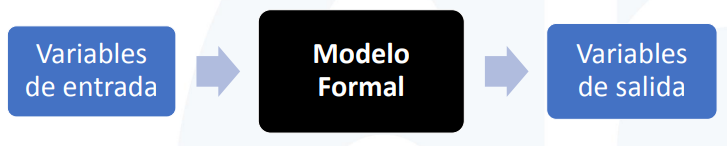
\includegraphics[keepaspectratio]{images/psicometria_IV-1.png}}

Los modelos formales, son un conjunto de relaciones ya definidas y no
necesariamente observables.

Un modelo necesariamente implica algún grado de reducción. Por esto no
son completamente exactos con problemas de la vida real, de hecho, se
trata de una idealización.

En términos lógicos los modelos pueden describir y/o predecir.

\textbf{El problema del modelo formal en psicometría:}

Los \textbf{modelos en disciplinas no sociales-humanas}, las denominadas
``ciencias duras'', tienen la ventaja de que se origina en información
observable, o que al menos puede ser medida con convenciones claras para
todos (cms., kgs., años).

En el \textbf{caso de la psicometría}, la información que nos interesa
medir no es observable, sino que es una \textbf{convención o constructo}
(por ejemplo: aprendizaje de matemática).

\textbf{Constructo}: un atributo cuya presencia podemos inferir a partir
de una serie de conductas (y actitudes, e incluso creencias).

\textbf{Pasos para medir un constructo:}

\begin{enumerate}
\def\labelenumi{\arabic{enumi}.}
\tightlist
\item
  Asignar un puntaje a una conducta observada.
\item
  Inferir un puntaje real a partir del puntaje observado.
\item
  Argumentar que el puntaje real refleja con certeza la ``cantidad'' de
  un constructo.
\end{enumerate}

El estudio de esta cadena de inferencias y sus implicancias mediante el
uso de modelos formales, en este caso, matemáticos y estadísticos se
realiza mediante las teorías psicométricas, que corresponden a modelos
estadísticos formales que relacionan mediciones de constructos con
mediciones de sus efectos observables.

\textbf{En la actualidad existen dos teorías ampliamente utilizadas:}

\begin{itemize}
\tightlist
\item
  Teoría Clásica de Tests (TCT).
\item
  Teoría de Respuesta al Ítem (IRT).
\end{itemize}

\chapter{Teoría Clasica de Test
(TCT)}\label{teoruxeda-clasica-de-test-tct}

Módulo teórico

\hfill\break

La teoría clásica de test es la forma más sencilla de analizar un test
que considera la información entregada por el test como un todo. En
otras palabras, utiliza el puntaje observado como una estimación
suficiente de la habilidad del individuo.

\section{\texorpdfstring{\textbf{Formulación
matemática}}{Formulación matemática}}\label{formulaciuxf3n-matemuxe1tica}

\[
X_{i} = V_{i} + E_{i}
\]

Donde:

\begin{itemize}
\tightlist
\item
  \(X_i\) = Puntaje observado.
\item
  \(V_i\) = Puntaje verdadero.
\item
  \(E_i\) = Error de medición.
\end{itemize}

\section{\texorpdfstring{\textbf{Supuestos de la
TCT}}{Supuestos de la TCT}}\label{supuestos-de-la-tct}

Primero es importante comprender \textbf{qué un supuesto} en una teoría
con un sustrato matemático.

\begin{itemize}
\tightlist
\item
  \textbf{Supuesto}: aquellas cosas que debemos dar por ciertas si
  queremos perseguir ese camino de demostración, en otras palabras, son
  \textbf{planteamientos sin demostración que quien utiliza la teoría
  debe dar por hecho}.
\end{itemize}

\textbf{Supuestos TCT:}

\begin{enumerate}
\def\labelenumi{\arabic{enumi}.}
\item
  La puntuación verdadera (\(V_i\)) es la esperanza matemática de la
  puntuación empírica.

  \begin{itemize}
  \item
    \textbf{Formulación MIDE}: Todos los ítems miden con error, pero
    estos errores se `cancelan' entre sí. El promedio de los errores de
    medición es cero.
  \item
    \textbf{Formulación matemática}: \(V = E(X)\)
  \item
    \textbf{Explicación en simple}: ``Se define la puntuación verdadera
    de una persona en un test como aquella puntuación que obtendría como
    media si se le pasase infinitas veces el test.'' (Muñiz 2010)
  \end{itemize}
\item
  No existe relación entre la cuantía de las puntuaciones verdaderas de
  las personas y el tamaño de los errores que afectan a esas
  puntuaciones.

  \begin{itemize}
  \item
    \textbf{Formuación MIDE}: Todos los ítems miden con error, pero
    estos errores no aumentan o disminuyen según el nivel de habilidad
    del evaluado: El error de medición no esta correlacionado con la
    habilidad del examinado (Puntaje verdadero).
  \item
    \textbf{Formulación matemática}: \(r(v,e) = 0\)
  \item
    \textbf{Explicación en simple}: ``El valor de la puntuación
    verdadera de una persona no tiene nada que ver con el error que
    afecta esa puntuación, es decir, puede haber puntuaciones verdaderas
    altas con errores bajos, o altos, no hay conexión entre el tamaño de
    la puntuación verdadera y el tamaño de los errores.''(Muñiz 2010)
  \end{itemize}
\item
  Los errores de medida de las personas en un test no están relacionados
  con los errores de medida en otro test distinto.

  \begin{itemize}
  \item
    \textbf{Formulación MIDE}: Todas las personas responden la prueba
    con error, pero este error es `único' para cada persona : Los
    errores de medición de dos estudiantes no están correlacionados
    entre sí.
  \item
    \textbf{Formulación matemática}: \(r(e_{j}, e_{k}) = 0\)
  \item
    \textbf{Explicación en simple}: ``No hay ninguna razón para pensar
    que los errores cometidos en una ocasión vayan a ocurrir en otra
    aplicación''.
  \end{itemize}
\end{enumerate}

\section{\texorpdfstring{\textbf{Análisis de Ítems y
pruebas}}{Análisis de Ítems y pruebas}}\label{anuxe1lisis-de-uxedtems-y-pruebas}

\textbf{Resumen estadístico TCT:}

\begin{center}
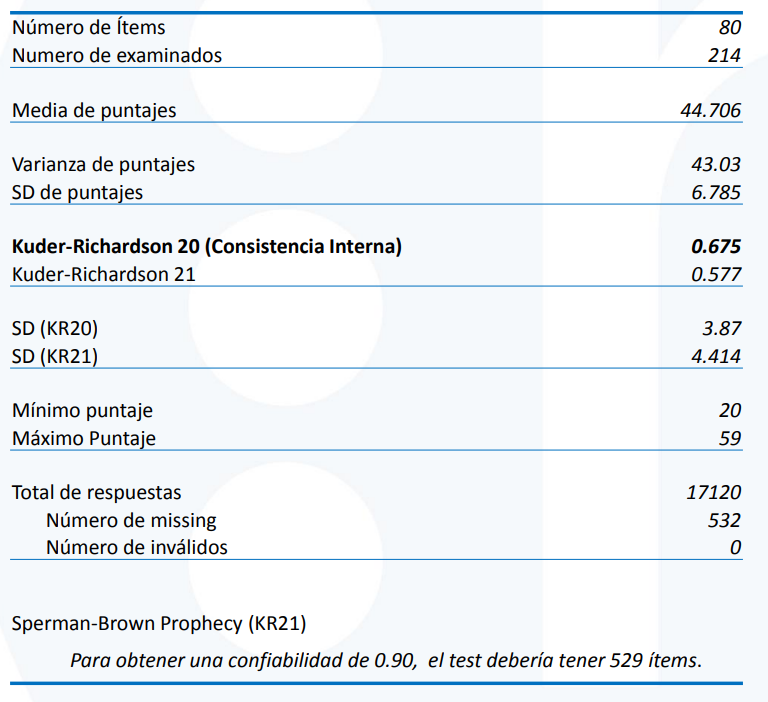
\includegraphics[width=0.6\linewidth,height=\textheight,keepaspectratio]{images/teoria_clasica_V-1.png}
\end{center}

\textbf{Cómo ordena las personas (por puntaje obtenido):}

\begin{center}
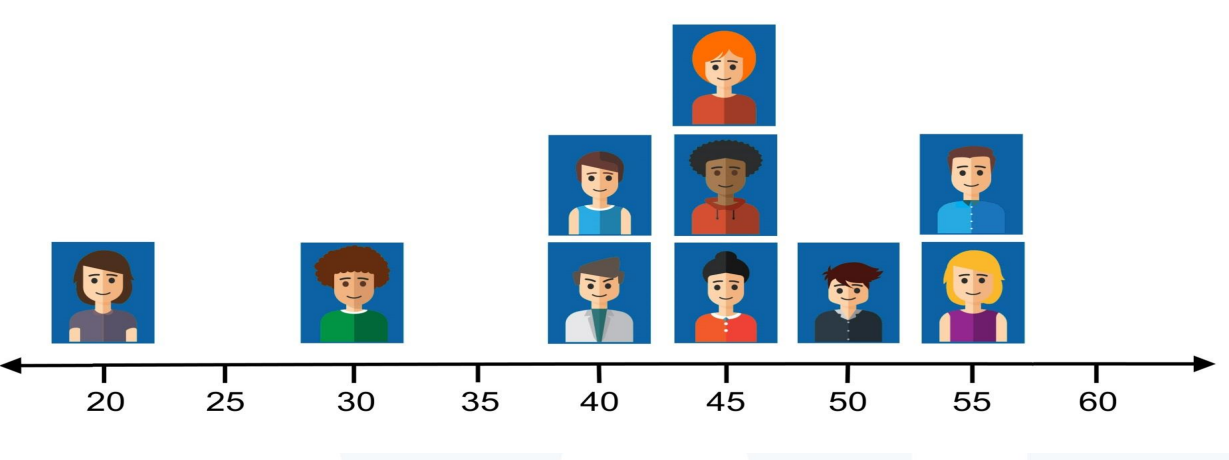
\includegraphics[width=0.6\linewidth,height=\textheight,keepaspectratio]{images/teoria_clasica_V-2.png}
\end{center}

\section{\texorpdfstring{\textbf{Error de
medición:}}{Error de medición:}}\label{error-de-mediciuxf3n}

\begin{itemize}
\tightlist
\item
  Como en todo modelamiento estadístico, es importante cuantificar el
  error aleatorio del proceso inferencial.
\item
  El error de medición permite cuantificar cuán preciso es el puntaje
  resultante de un test.
\item
  Se expresa en la misma escala de las puntuaciones observadas.
\item
  Permite construir un Intervalo de Confianza para el puntaje verdadero.
\item
  Se relaciona de forma inversa con la confiabilidad.
\end{itemize}

\section{\texorpdfstring{\textbf{Ventajas y
Limitaciones}}{Ventajas y Limitaciones}}\label{ventajas-y-limitaciones}

\textbf{Ventajas:}

\begin{itemize}
\tightlist
\item
  Es fácil de interpretar.
\item
  Los cálculos son sencillos de realizar en cualquier computador y
  software estadístico.
\end{itemize}

\textbf{Limitaciones:}

\begin{itemize}
\tightlist
\item
  La estimación de habilidad de los examinados se basa en sus respuestas
  al test como un todo, y no en el funcionamiento particular de los
  ítems.
\item
  Estimaciones de habilidad dependen de los ítems administrados y de la
  muestra utilizada.
\item
  Los parámetros de los ítems dependen de la muestra en que son
  estimados.
\item
  El error de estimación se basa en el comportamiento de un grupo.
\item
  Parámetros de los ítems y estimaciones de habilidad se expresan en
  escalas diferentes.
\end{itemize}

\section{Estadígrafos relevantes en
TCT}\label{estaduxedgrafos-relevantes-en-tct}

En este apartado se presentará una introducción conceptual a cada
estadígrafo. Más adelante, en capitulos de profundización, se abordarán
los detalles matemáticos y limitaciones de estos estadígrafos.

\begin{itemize}
\item
  \textbf{Alpha de Cronbach}: Es una medida de la consistencia interna
  de prueba, es decir, qué tan relacionados están los ítems de una
  prueba si los consideramos como un conjunto.
\item
  \textbf{Tasa de omisión}: Es la proporción de personas que omite cada
  ítem. Se puede leer de forma aislada, donde se verifica que un ítem
  singular tenga una omisión baja. También se puede ver de forma
  posicional, donde se estudia el recorrido que hizo el alumno por los
  ítemes ordenados para verificar si existe un patrón de omisión.
\item
  \textbf{Proporción de respuesta}: Es la proporción de personas que
  marca cada una de las respuestas. La proporción de respuestas de la
  alternativa que figura como respuesta correcta es idéntico a la
  dificultad del ítem.
\item
  \textbf{Biseriales}: Son diferentes medidas posibles de correlación
  entre puntaje total obtenido por los alumnos que marcaron esa
  alternativa y los alumnos que no marcaron la alternativa. La biserial
  de la respuesta que figura como correcta es idéntico a la
  discriminación del ítem.
\item
  \textbf{Dificultad}: Es la proporción de personas que tiene correcto
  el ítem.
\item
  \textbf{Discriminación}: Es una medida de la diferencia en puntaje
  total de alumnos con buen y mal rendimiento en un ítem específico.
  Existen diversos métodos para calcularla en teoría clásica.
\end{itemize}

\section{Dificultad}\label{dificultad}

Se mide para cada ítem como la proporción de personas que tuvieron ese
ítem correcto.

\[
Dificultad_i = \frac{cantidad\ de\ respuestas\ correctas_i}{cantidad\ total\ de\ respuestas}
\]

Donde:

\begin{itemize}
\item
  \(Dificultad_i\) = dificultad del ítem i.
\item
  \(cantidad\ de\ respuestas\ correctas_i\) = cantidad de respuestas
  correctas para el ítem i.
\end{itemize}

\section{Discriminación}\label{discriminaciuxf3n}

Conceptualmente indica la capacidad de la pregunta de diferenciar entre
personas con alta y baja habilidad del constructo que se pretende medir.

Se puede medir de diversas formas:

\textbf{Forma Básica:}

\[
Discriminación_i = prop_i(p_i=1)\ de\ puntajes\ totales\ altos\ - prop_i(p_i=1)\ de\ puntajes\ totales\ bajos
\]

Donde:

\begin{itemize}
\tightlist
\item
  \(prop_i(x_i = 1)\) = proporción de respuestas correctas para el ítem
  i.
\end{itemize}

\textbf{Correlación item\_total:}

\[
Discriminación_i = p_{it} = \frac{Cov(i,t)}{\sigma_i\sigma_t}
\]

Donde:

\begin{itemize}
\item
  \(Discriminación_i\) = Discriminación del ítem i.
\item
  \(i\) = Puntaje en el ítem i del sujeto.
\item
  \(t\) = Puntaje total obtenido por el sujeto.
\item
  \(P_{it}\) es la correlación de Pearson entre i y t.
\end{itemize}

\textbf{Punto biserial:}

\begin{longtable}[]{@{}
  >{\raggedright\arraybackslash}p{(\linewidth - 2\tabcolsep) * \real{0.5000}}
  >{\raggedright\arraybackslash}p{(\linewidth - 2\tabcolsep) * \real{0.5000}}@{}}
\toprule\noalign{}
\begin{minipage}[b]{\linewidth}\raggedright
Con cantidad de casos
\end{minipage} & \begin{minipage}[b]{\linewidth}\raggedright
Con probabilidades
\end{minipage} \\
\midrule\noalign{}
\endhead
\bottomrule\noalign{}
\endlastfoot
\(
r_{pb} = \frac{\bar{x}_{p = 1} - \bar{x}_{p = 0}}{\sigma_T} \sqrt{\frac{n_1 . n_2}{n^2}}
\) & \(
r_{pb} = \frac{\bar{x}_{p = 1} - \bar{x}_{p = 0}}{\sigma_T} \sqrt{pq}
\) \\
\begin{minipage}[t]{\linewidth}\raggedright
Donde:

\begin{itemize}
\item
  \(r_{pb}\) = Punto biserial.
\item
  \(\bar{x}_{p = 1}\) = media de puntaje total de los sujetos que
  tuvieron el ítem \textbf{correcto}.
\item
  \(\bar{x}_{p = 0}\) = media de puntaje total de los sujetos que
  tuvieron el ítem \textbf{incorrecto}.
\item
  \(\sigma_T\) = desviación estándar de los puntajes totales entre
  sujetos.
\item
  \(n_1\) = cantidad de personas que \textbf{aprobaron} el ítem.
\item
  \(n_2\) = cantidad de personas que \textbf{reprobaron} el ítem.
\item
  \(n\) = número total de personas que rindieron el ítem.
\end{itemize}
\end{minipage} & \begin{minipage}[t]{\linewidth}\raggedright
Donde:

\begin{itemize}
\item
  \(r_{pb}\) = Punto biserial.
\item
  \(\bar{x}_{p = 1}\) = media de puntaje total de los sujetos que
  tuvieron el ítem \textbf{correcto}.
\item
  \(\bar{x}_{p = 0}\) = media de puntaje total de los sujetos que
  tuvieron el ítem \textbf{incorrecto}.
\item
  \(\sigma_T\) = desviación estándar de los puntajes totales entre
  sujetos.
\item
  \(p\) = probabilidad de tener la pregunta \textbf{correcta}.
\item
  \(q\) = probabilidad de tener la pregunta \textbf{incorrecta}.
\end{itemize}
\end{minipage} \\
\end{longtable}

Existen estratégicas matemáticas para obtener punto-biseriales y
correlaciones item-test con más información. Algunas son:

\begin{itemize}
\item
  Para el puntaje total, NO considerar el puntaje del ítem evaluado, es
  decir, si la prueba tenía 15 puntos máximo para efectos de este
  análisis tiene 14. Esto es lo que se conoce como un cálculo de
  biserial item-reminder.
\item
  Algunos cálculos de biserial en lugar de calcular la diferencia de p=1
  - p=0, utilizan la media de todos los sujetos de esta forma: p=1ó0 -
  p=0.
\end{itemize}

\section{Output tipo de TCT de la
unidad}\label{output-tipo-de-tct-de-la-unidad}

\subsection{\texorpdfstring{\textbf{Dificultad:}}{Dificultad:}}\label{dificultad-1}

\begin{tcolorbox}[enhanced jigsaw, opacityback=0, bottomrule=.15mm, rightrule=.15mm, leftrule=.75mm, coltitle=black, colbacktitle=quarto-callout-tip-color!10!white, left=2mm, title=\textcolor{quarto-callout-tip-color}{\faLightbulb}\hspace{0.5em}{Tip}, bottomtitle=1mm, toprule=.15mm, colframe=quarto-callout-tip-color-frame, breakable, titlerule=0mm, toptitle=1mm, arc=.35mm, colback=white, opacitybacktitle=0.6]

Cuando se realiza un análisis de dificultad se tiene que plantear un
rango de corte, generalmente simétrico entre ambos extremos. Este rango
varía según las exigencias y características de la
prueba/población/propósito.

Para este ejemplo se utiliza un estándar de algunas pruebas
internacionales de 0.15 puntos, entonces:

\begin{itemize}
\item
  Menor a 0.15: ítem difícil.
\item
  Mayor a 0.85: ítem fácil.
\end{itemize}

\end{tcolorbox}

\section{Bruto}

\begin{center}
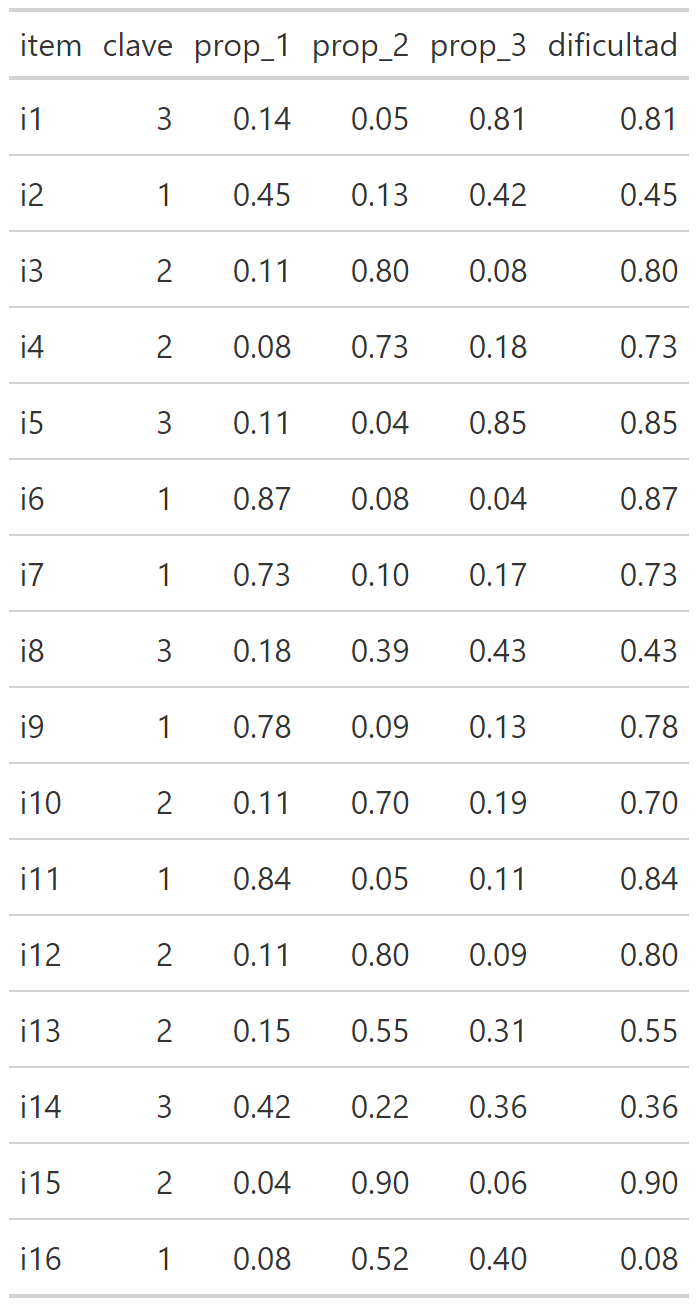
\includegraphics[width=0.6\linewidth,height=\textheight,keepaspectratio]{images/teoria_clasica_diff_blank.png}
\end{center}

\section{Fácil}

\begin{center}
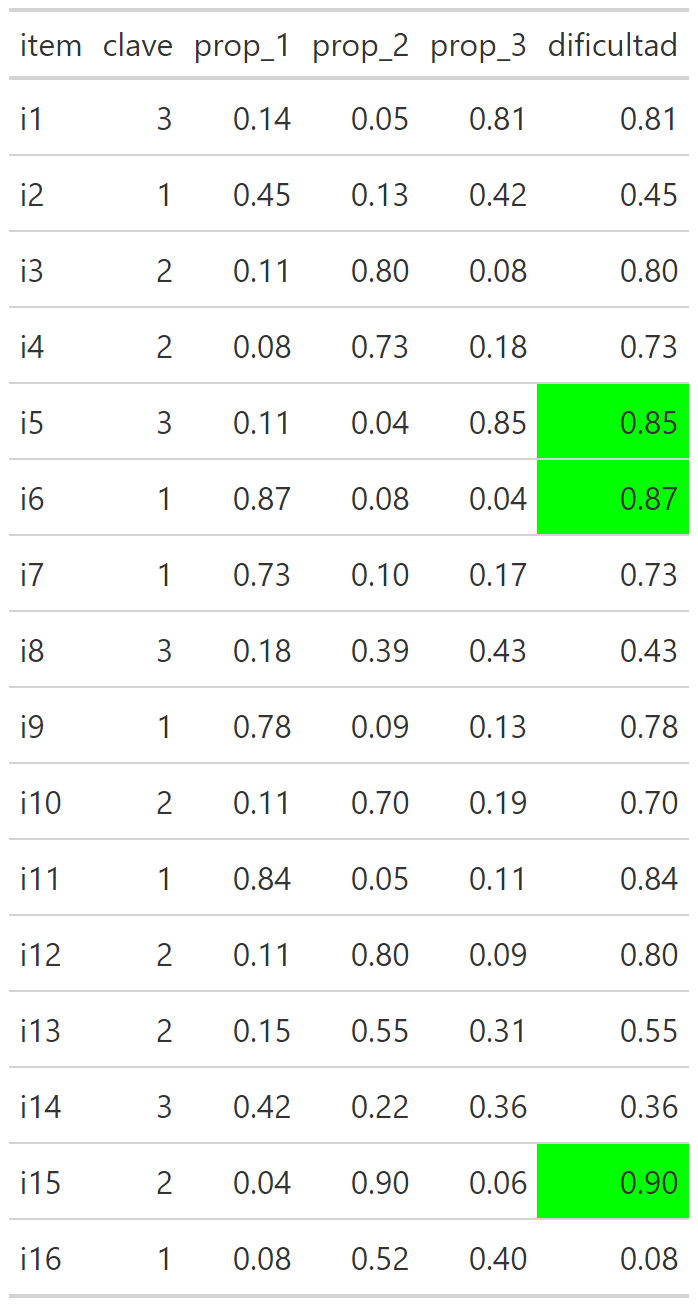
\includegraphics[width=0.6\linewidth,height=\textheight,keepaspectratio]{images/teoria_clasica_diff_facil.png}
\end{center}

\section{Medio}

\begin{center}
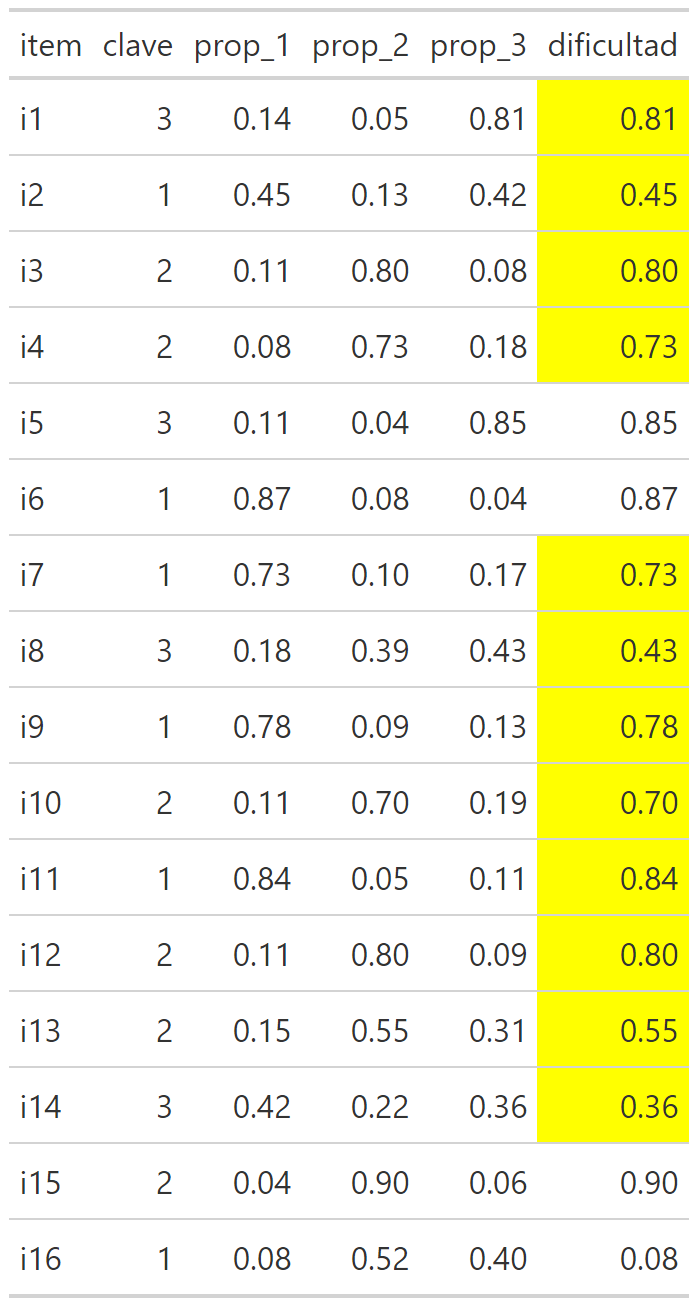
\includegraphics[width=0.6\linewidth,height=\textheight,keepaspectratio]{images/teoria_clasica_diff_medio.png}
\end{center}

\section{Difícil}

\begin{center}
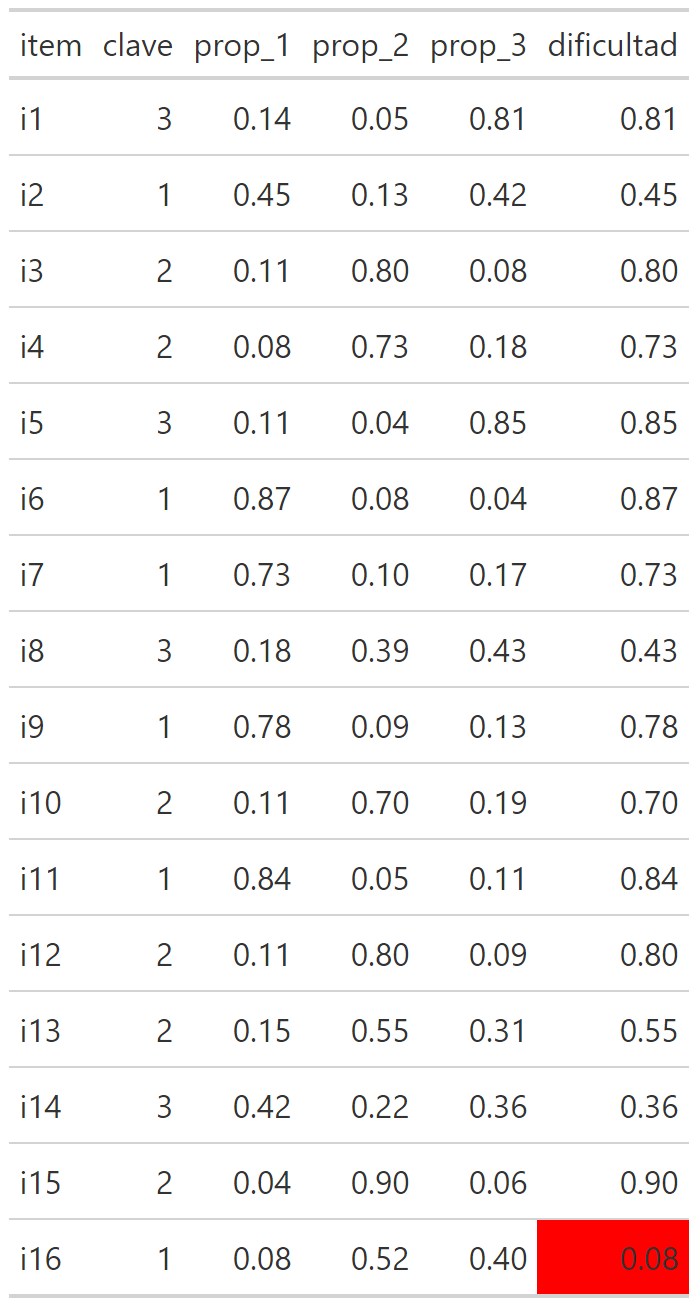
\includegraphics[width=0.6\linewidth,height=\textheight,keepaspectratio]{images/teoria_clasica_diff_dificil.png}
\end{center}

\section{Todos}

\begin{center}
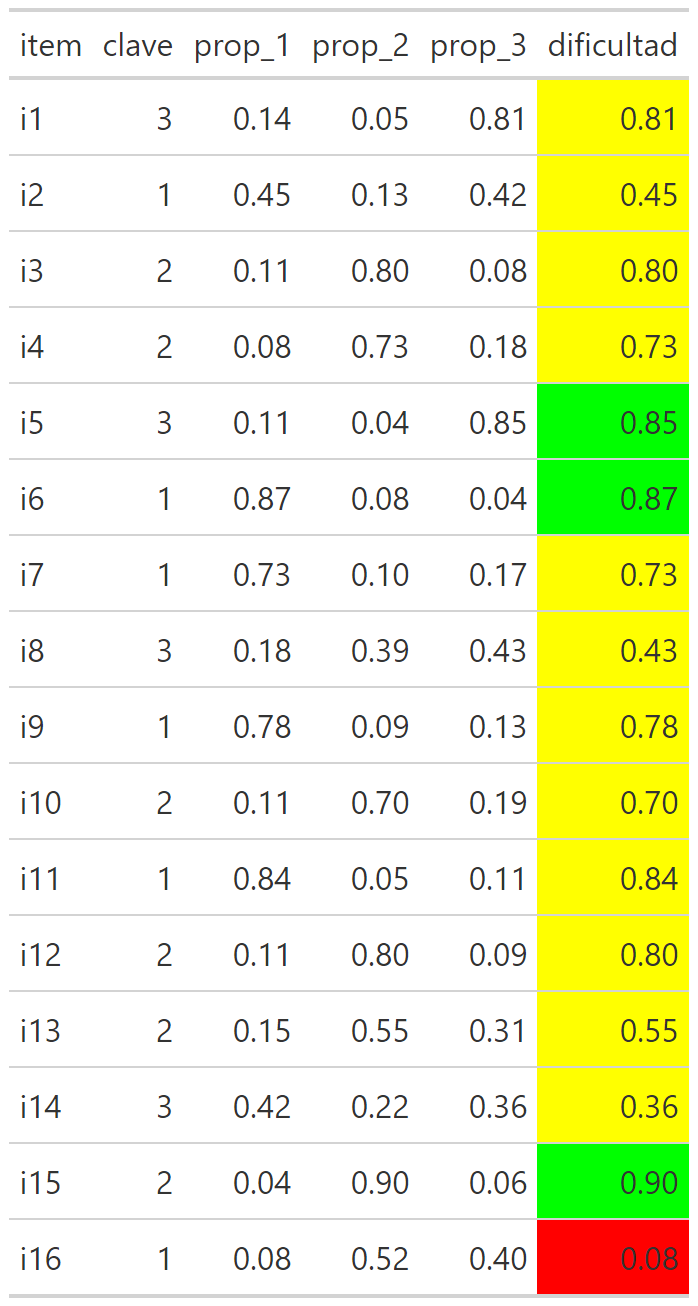
\includegraphics[width=0.6\linewidth,height=\textheight,keepaspectratio]{images/teoria_clasica_diff_all.png}
\end{center}

\subsection{\texorpdfstring{\textbf{Discriminación}}{Discriminación}}\label{discriminaciuxf3n-1}

\begin{tcolorbox}[enhanced jigsaw, opacityback=0, bottomrule=.15mm, rightrule=.15mm, leftrule=.75mm, coltitle=black, colbacktitle=quarto-callout-tip-color!10!white, left=2mm, title=\textcolor{quarto-callout-tip-color}{\faLightbulb}\hspace{0.5em}{Tip}, bottomtitle=1mm, toprule=.15mm, colframe=quarto-callout-tip-color-frame, breakable, titlerule=0mm, toptitle=1mm, arc=.35mm, colback=white, opacitybacktitle=0.6]

Cuando se analiza la discriminación se suelen utilizar estándares
similares a la evaluación de una correlación, entonces:

\begin{itemize}
\item
  Mayor a 0.3: discriminación suficiente.
\item
  Menor a 0.3: discriminación insuficiente.
\end{itemize}

Dicho lo anterior, a veces, considerando otras ventajas psicométricas
que tenga un ítem se permiten discriminaciones en un rango 0.15 - 0.3 a
las que llamaremos discriminación media.

\end{tcolorbox}

\section{Bruto}

\begin{center}
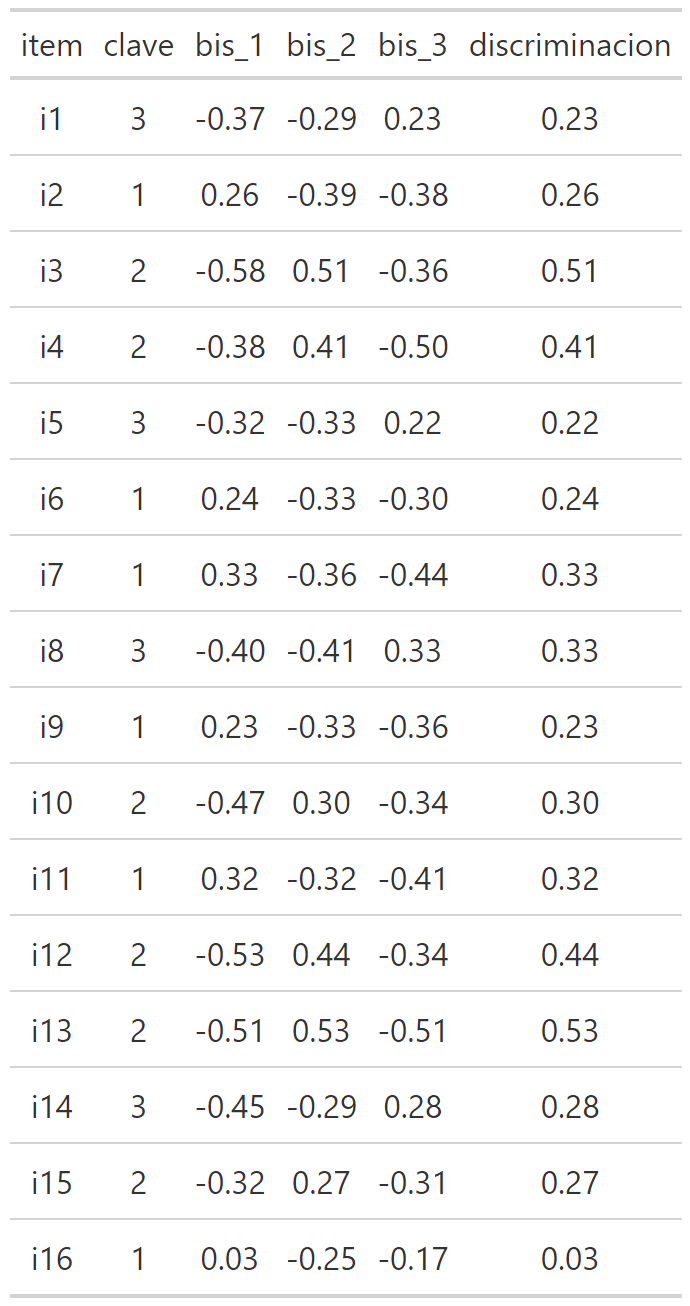
\includegraphics[width=0.6\linewidth,height=\textheight,keepaspectratio]{images/teoria_clasica_disc_blank.png}
\end{center}

\section{Suficiente}

\begin{center}
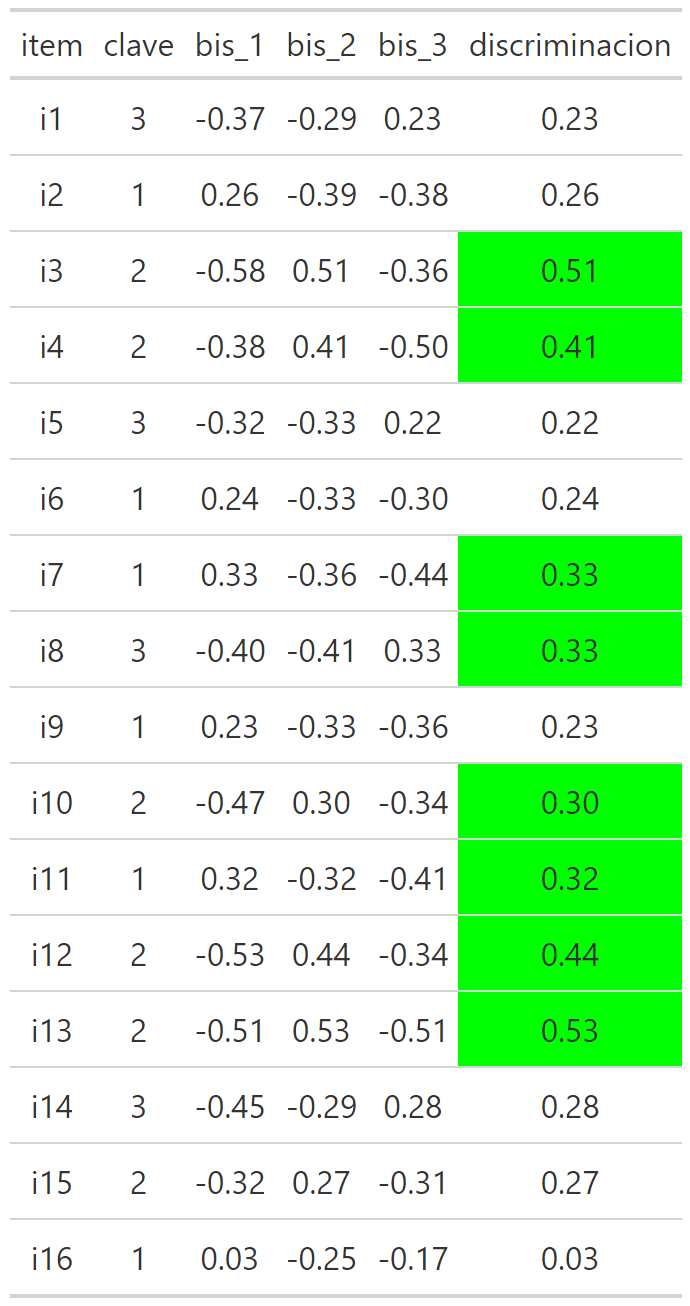
\includegraphics[width=0.6\linewidth,height=\textheight,keepaspectratio]{images/teoria_clasica_disc_buena.png}
\end{center}

\section{Media}

\begin{center}
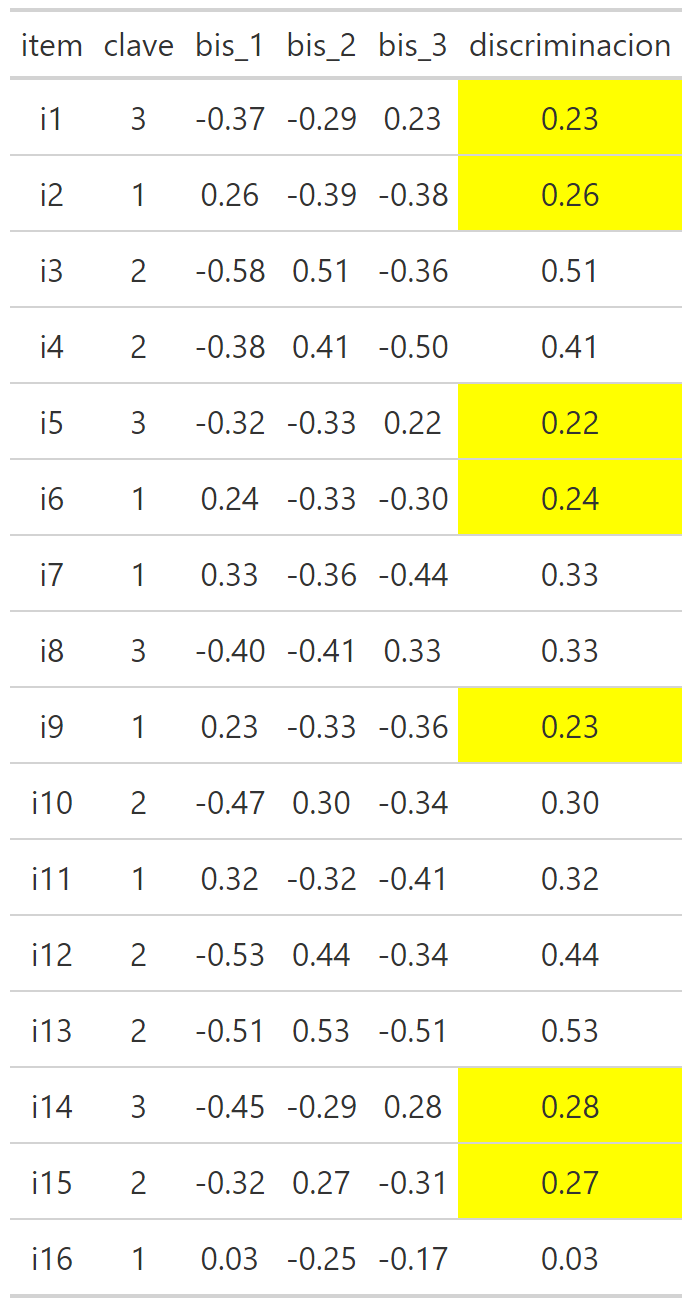
\includegraphics[width=0.6\linewidth,height=\textheight,keepaspectratio]{images/teoria_clasica_disc_medio.png}
\end{center}

\section{Insuficiente}

\begin{center}
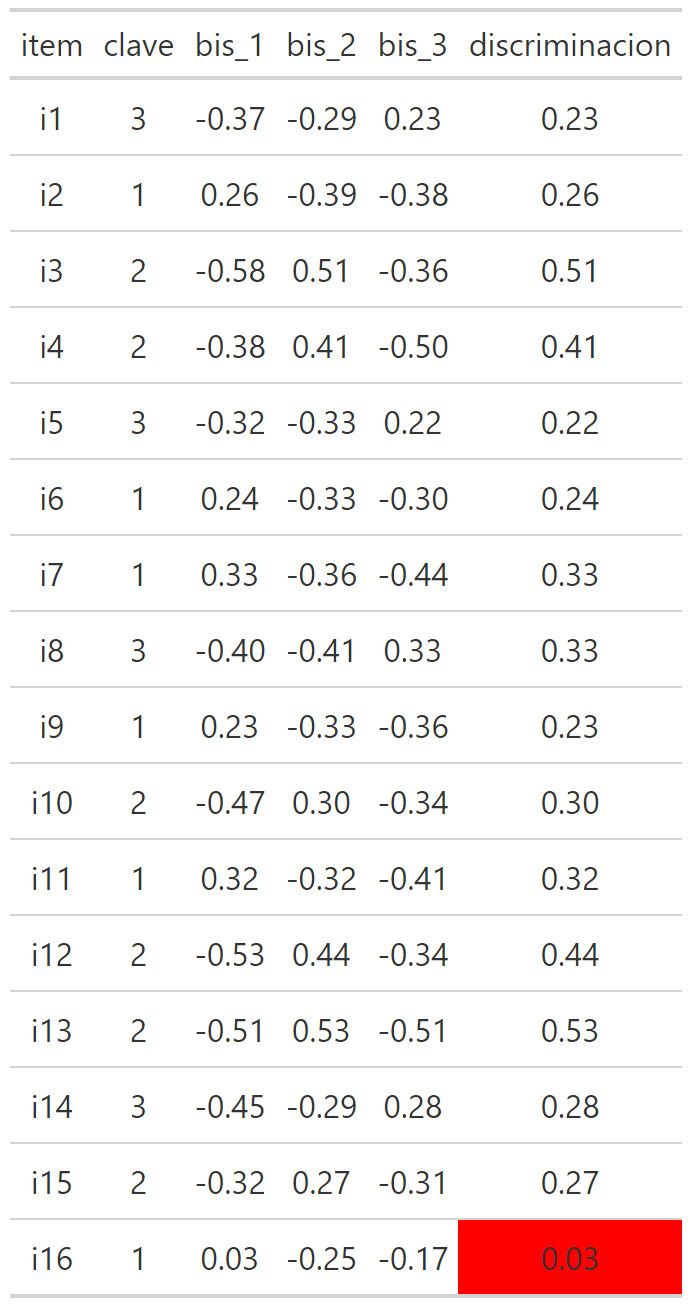
\includegraphics[width=0.6\linewidth,height=\textheight,keepaspectratio]{images/teoria_clasica_disc_insuficiente.png}
\end{center}

\section{Todos}

\begin{center}
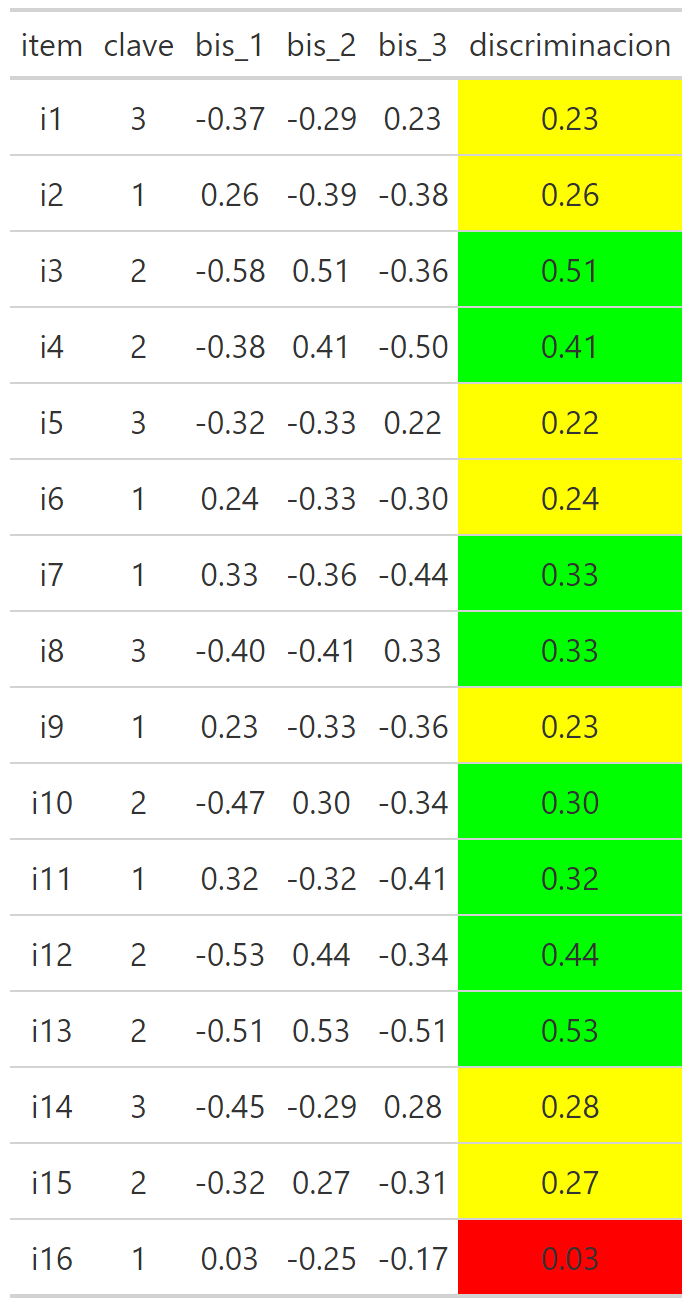
\includegraphics[width=0.6\linewidth,height=\textheight,keepaspectratio]{images/teoria_clasica_disc_all.png}
\end{center}

\chapter{Teoría de Respuesta al Ítem
(IRT)}\label{teoruxeda-de-respuesta-al-uxedtem-irt}

Módulo teórico

\hfill\break

IRT es una teoría que surge como respuesta a algunas de las carencias
que presentaba la teoría clásica, especialmente vinculada a la noción de
utilizar el puntaje total como una medida apropiada de habilidad.

En la lógica IRT podríamos decir que cada ítem de la prueba es un mundo
aparte y su análisis se realiza de manera aislada. Una vez teniendo
claras las características del ítem podemos ``puntuar'' a los sujetos
utilizando algunas técnicas.

Para entender la formulación matemática del IRT se vuelve necesario una
pequeña introducción las funciones exponenciales y la constante Euler
(\(e\)).

\textbf{INSERTAR INTRODUCCION A EULER}

\(z\)

\section{\texorpdfstring{\textbf{Formulación matemática
simple}}{Formulación matemática simple}}\label{formulaciuxf3n-matemuxe1tica-simple}

\begin{longtable}[]{@{}
  >{\raggedright\arraybackslash}p{(\linewidth - 2\tabcolsep) * \real{0.5000}}
  >{\raggedright\arraybackslash}p{(\linewidth - 2\tabcolsep) * \real{0.5000}}@{}}
\toprule\noalign{}
\begin{minipage}[b]{\linewidth}\raggedright
Forma 1
\end{minipage} & \begin{minipage}[b]{\linewidth}\raggedright
Forma 2
\end{minipage} \\
\midrule\noalign{}
\endhead
\bottomrule\noalign{}
\endlastfoot
\(
P(y = 1|z) = \frac{e^z}{1+e^z}
\) & \(
P(y = 1|z) = \frac{1}{1+e^{-z}}
\) \\
\begin{minipage}[t]{\linewidth}\raggedright
Donde:

\begin{itemize}
\item
  \(P(y=1|z)\) = La probabilidad de que el resultado sea = 1, dado z
  (condición bayesiana).
\item
  \(e\) = constante de euler.
\item
  \(z\) = condición.
\end{itemize}
\end{minipage} & \begin{minipage}[t]{\linewidth}\raggedright
Donde:

\begin{itemize}
\item
  \(P(y=1|z)\) = La probabilidad de que el resultado sea = 1, dado z
  (condición bayesiana).
\item
  \(e\) = constante de euler.
\item
  \(z\) = condición.
\end{itemize}
\end{minipage} \\
\end{longtable}

En general se utiliza la forma 1 ya que es más clara de visualizar.

Lo que va a cambiar entre los modelos IRT es qué es el z.

\section{\texorpdfstring{\textbf{Supuestos de
IRT}}{Supuestos de IRT}}\label{supuestos-de-irt}

\begin{enumerate}
\def\labelenumi{\arabic{enumi}.}
\item
  \textbf{Monotonía}: a medida que aumenta el nivel de habilidad en la
  dimensión medida mayor es la probabilidad de responder correctamente.
\item
  \textbf{Unidimensionalidad}: existe una variable latente dominante que
  se está midiendo y esta latente es lo que explica las respuestas
  observadas para cada ítem.
\item
  \textbf{Independencia local}: las respuestas entregadas para los ítems
  son independientes entre sí dada un cierto nivel de habilidad, es
  decir, responder bien un ítem no te va a ayudar a responder bien otro
  de los ítems.
\item
  \textbf{Invarianza}: no existen razones para pensar que existen
  manifestaciones distintas de la habilidad medida entre personas, es
  decir, la misma función aplicaría para toda la población.
\end{enumerate}

\section{\texorpdfstring{\textbf{Introducción a los
parámetros}}{Introducción a los parámetros}}\label{introducciuxf3n-a-los-paruxe1metros}

Para reemplazar la variable z, mencionada anteriormente en la
formulación matemática, existen 5 parámetros que alteran la curva del
modelo de alguna manera.

Esos 5 parámetros se diferencian en 2 tipos:

\begin{itemize}
\item
  Parámetros de los evaluados (p).
\item
  Parámetros de los ítems (i).
\end{itemize}

\textbf{Parámetros de los evaluados}

Es solo 1 parámetro que se le llama habilidad y es simbolizado como
\(\theta_p\).

\textbf{Parámetros de los ítems}

\begin{enumerate}
\def\labelenumi{\arabic{enumi}.}
\tightlist
\item
  \textbf{Dificultad} (\(b_i\)):

  \begin{itemize}
  \item
    \textbf{Matemáticamente}: altera dónde está el centro de la curva,
    es decir, el nivel de habilidad (\(\theta\)) donde la probabilidad
    de acierto es 0.5.
  \item
    \textbf{Conceptualmente}: marca la habilidad que necesitaría una
    persona para tener más posibilidades de tener la respuesta correcta
    que incorrecta \(P(correcta)>P(incorrecta)\).
  \end{itemize}
\item
  \textbf{Discriminación} (\(a_i\)):

  \begin{itemize}
  \item
    \textbf{Matemáticamente}: altera la pendiente de la curva, es decir,
    a mayor discriminación se necesita un mayor nivel de habilidad para
    responder la respuesta correctamente.
  \item
    \textbf{Conceptualmente}: Un ítem que discrimina mejor diferencia
    mejor entre un alumno de alta habilidad que de baja habilidad.
  \end{itemize}
\item
  \textbf{Adivinación} (\(c_i\)):

  \begin{itemize}
  \item
    \textbf{Matemáticamente}: altera la altura inicial de la curva, es
    decir, el punto donde el eje ``x'' es 0 genera un ``y'' mayor a 0.
  \item
    \textbf{Conceptualmente}: como queremos explicar la probabilidad de
    acierto dado el nivel de habilidad de la persona de forma lo más
    aislada posible debemos descartar o considerar en la ecuación la
    posibilidad de que el alumno simplemente le haya achuntado. Esto se
    realiza ``regalandole'' a todos los sujetos una pequeña probabilidad
    de base.
  \item
    Otra forma de pensar este parámetro es que van a existir casos de
    \textbf{falsos positivos}, donde vas a tener la pregunta correcta
    sin tener la habilidad suficiente para tener esa pregunta correcta,
    por lo tanto, se aumenta un poco la probabilidad basal para
    considerar este efecto.
  \end{itemize}
\item
  \textbf{Inatención} (\(d_i\)): altera la altura final de la curva (el
  techo).

  \begin{itemize}
  \item
    \textbf{Matemáticamente}: altera la altura final de la curva, es
    decir, el punto donde el eje ``x'' es infinito genera un ``y'' menor
    a 1.
  \item
    \textbf{Conceptualmente}: como queremos explicar la probabilidad de
    acierto dado el nivel de habilidad de la persona de forma lo más
    aislada posible debemos descartar o considerar en la ecuación la
    posibilidad de que el alumno no esté prestando atención por algún
    factor externo a su habilidad. Esto se realiza ``quitandole'' a
    todos los sujetos una pequeña probabilidad de base.
  \item
    Otra forma de pensar este parámetro es que van a existir casos de
    \textbf{falsos negativos}, donde vas a tener la pregunta incorrecta
    teniendo la habilidad suficiente para tener esa pregunta correcta,
    por lo tanto, se aumenta un poco la probabilidad basal para
    considerar este efecto.
  \end{itemize}
\end{enumerate}

Dependiendo de cuántos parámetros tenga el modelo se denominan como 1PL,
2PL, 3PL o 4PL.

Una idea que es importante para entender estos modelos es la diferencia
en cuando un parámetro actúa como variable y como valor constante. La
realidad oculta de los modelos es que todos poseen todos los parámetros
en sus equaciones, la diferencia real entre los modelos es si estos
parámetros son constantes o variables.

Al presentar los modelos a continuación se presentará la versión
reducida con solo los parámetros variables y la versión completa que
incluye los parámetros constantes implícitos.

\section{Formula completa IRT hasta
4PL}\label{formula-completa-irt-hasta-4pl}

\[
P(y=1|\theta_p;b_i,a_i,c_i,d_i) = c_i + (d_i-c_i)\left(\frac{e^{a_i(\theta_p-b_i)}}{1 + e^{a_i(\theta_p-b_i)}}\right)
\]

Donde:

\begin{itemize}
\tightlist
\item
  \(P(y=1|\theta_p;b_i,a_i,c_i,d_i)\) = probabilidad de tener el ítem
  correcto considerando el nivel de habilidad del estudiante p; y la
  dificultad, discriminación, posibilidad de adivinación e inatención
  para el ítem i.
\item
  \(\theta_p\) = habilidad del estudiante p.
\item
  \(a_i\)= discriminación del ítem i.
\item
  \(b_i\)= dificultad del ítem i.
\item
  \(c_i\)= posibilidad de adivinación para el ítem i.
\item
  \(d_i\)= posibilidad de inatención para el ítem i.
\end{itemize}

\section{1PL - Modelo Rasch}\label{pl---modelo-rasch}

\begin{longtable}[]{@{}
  >{\raggedright\arraybackslash}p{(\linewidth - 2\tabcolsep) * \real{0.5000}}
  >{\raggedright\arraybackslash}p{(\linewidth - 2\tabcolsep) * \real{0.5000}}@{}}
\toprule\noalign{}
\begin{minipage}[b]{\linewidth}\raggedright
Versión reducida
\end{minipage} & \begin{minipage}[b]{\linewidth}\raggedright
Versión completa
\end{minipage} \\
\midrule\noalign{}
\endhead
\bottomrule\noalign{}
\endlastfoot
\(
 P(y = 1|\theta_p;b_i) = \frac{e^{(\theta_p-b_i)}}{1+e^{(\theta_p-b_i)}}
\) & \(
P(y=1|\theta_p;b_i) = 0 + (1-0)\left(\frac{e^{1(\theta_p-b_i)}}{1 + e^{1(\theta_p-b_i)}}\right)
\) \\
\begin{minipage}[t]{\linewidth}\raggedright
Donde:

\begin{itemize}
\item
  \(P(y=1|\theta_p;b_i)\) = Probabilidad de tener el ítem correcto
  considerando el nivel de habilidad del estudiante p y la dificultad
  del ítem i.
\item
  \(e\) = constante de euler.
\item
  \(\theta_p\) = nivel de habilidad de la dimensión medida del
  estudiante/participante p.
\item
  \(b_i\) = dificultad del ítem i.
\end{itemize}
\end{minipage} & \begin{minipage}[t]{\linewidth}\raggedright
Donde:

\begin{itemize}
\item
  \(P(y=1|\theta_p;b_i)\) = Probabilidad de tener el ítem correcto
  considerando el nivel de habilidad del estudiante p y la dificultad
  del ítem i.
\item
  \(e\) = constante de euler.
\item
  \(\theta_p\) = nivel de habilidad de la dimensión medida del
  estudiante/participante p.
\item
  \(b_i\) = dificultad del ítem i.
\item
  \(a_i\) = 1
\item
  \(c_i\) = 0
\item
  \(d_i\) = 1
\end{itemize}
\end{minipage} \\
\end{longtable}

Existe una diferencia sutil entre ejecutar un modelo 1PL y Rasch que se
aprecia en las siguientes ecuaciones:

\begin{longtable}[]{@{}
  >{\centering\arraybackslash}p{(\linewidth - 2\tabcolsep) * \real{0.2492}}
  >{\centering\arraybackslash}p{(\linewidth - 2\tabcolsep) * \real{0.7508}}@{}}
\toprule\noalign{}
\begin{minipage}[b]{\linewidth}\centering
Rasch
\end{minipage} & \begin{minipage}[b]{\linewidth}\centering
1PL
\end{minipage} \\
\midrule\noalign{}
\endhead
\bottomrule\noalign{}
\endlastfoot
\(                                     
   P(y = 1|\theta_p,b_i) = \frac{e^{1(\theta_p-b_i)}}{1+e^{1(\theta_p-b_i)}} 
                                      \) &
\(                                                                        P(y = 1|\theta_p,b_i) = \frac{e^{1.7(\theta_p-b_i)}}{1+e^{1.7(\theta_p-b_i)}}                                                                          \) \\
\end{longtable}

El \textbf{modelo 1PL} el parámetro \textbf{discriminación} es
constante, pero puede tomar \textbf{cualquier} \textbf{valor} (1.7 en el
ejemplo).

El \textbf{modelo Rasch} siempre va a poseer \textbf{discriminación =
1}.

\section{2PL}\label{pl}

\begin{longtable}[]{@{}
  >{\raggedright\arraybackslash}p{(\linewidth - 2\tabcolsep) * \real{0.5000}}
  >{\raggedright\arraybackslash}p{(\linewidth - 2\tabcolsep) * \real{0.5000}}@{}}
\toprule\noalign{}
\begin{minipage}[b]{\linewidth}\raggedright
Versión reducida
\end{minipage} & \begin{minipage}[b]{\linewidth}\raggedright
Versión completa
\end{minipage} \\
\midrule\noalign{}
\endhead
\bottomrule\noalign{}
\endlastfoot
\(
P(y=1|\theta_p;b_i,a_i) = \frac{e^{a_i(\theta_p-b_i)}}{1 + e^{a_i(\theta_p-b_i)}}
\) & \(
P(y=1|\theta_p;b_i,c_i) = 0 + (1-0)\left(\frac{e^{a_i(\theta_p-b_i)}}{1 + e^{a_i(\theta_p-b_i)}}\right)
\) \\
\begin{minipage}[t]{\linewidth}\raggedright
Donde:

\begin{itemize}
\item
  \(P(y=1|\theta_p;b_i,c_i)\) = Probabilidad de tener el ítem correcto
  considerando el nivel de habilidad del estudiante p; y la dificultad y
  discriminación del ítem i.
\item
  \(e\) = constante de euler.
\item
  \(\theta_p\) = nivel de habilidad de la dimensión medida del
  estudiante/participante p.
\item
  \(b_i\) = dificultad del ítem i.
\item
  \(a_i\) = discriminación del ítem i.
\end{itemize}
\end{minipage} & \begin{minipage}[t]{\linewidth}\raggedright
Donde:

\begin{itemize}
\item
  \(P(y=1|\theta_p;b_i,c_i)\) = Probabilidad de tener el ítem correcto
  considerando el nivel de habilidad del estudiante p; y la dificultad y
  discriminación del ítem i.
\item
  \(e\) = constante de euler.
\item
  \(\theta_p\) = nivel de habilidad de la dimensión medida del
  estudiante/participante p.
\item
  \(b_i\) = dificultad del ítem i.
\item
  \(a_i\) = discriminación del ítem i.
\item
  \(c_i\) = 0
\item
  \(d_i\) = 1
\end{itemize}
\end{minipage} \\
\end{longtable}

\section{3PL}\label{pl-1}

En 3PL se presenta solo la fórmula del modelo ya que se necesita mostrar
el 1 asociado a la inatención siempre.

\[
P(y=1|\theta_p;b_i,a_i,c_i) = c_i + (1-c_i) \left(\frac{e^{a_i(\theta_p-b_i)}}{1 + e^{a_i(\theta_p-b_i)}}\right)
\]

Donde:

\begin{itemize}
\item
  \(P(y=1|\theta_p;b_i,a_i,c_i)\) = Probabilidad de tener el ítem
  correcto considerando el nivel de habilidad del estudiante p; y la
  dificultad, discriminación y posibilidad de adivinación para el ítem
  i.
\item
  \(e\) = constante de euler.
\item
  \(\theta_p\) = nivel de habilidad de la dimensión medida del
  estudiante/participante p.
\item
  \(b_i\) = dificultad del ítem i.
\item
  \(a_i\) = discriminación del ítem i.
\item
  \(c_i\) = adivinación del ítem i.
\end{itemize}

\section{Curvas características de los ítem
(ICC)}\label{curvas-caracteruxedsticas-de-los-uxedtem-icc}

\begin{itemize}
\item
  \textbf{Eje x}: escala de habilidad de los sujetos (\(\theta\)) -
  unidad logit.
\item
  \textbf{Eje y}: Probabilidad de marcar correcto el ítem.
\end{itemize}

\section{Curvas de información}\label{curvas-de-informaciuxf3n}

\textbf{Para los ítems:}

\begin{longtable}[]{@{}
  >{\raggedright\arraybackslash}p{(\linewidth - 4\tabcolsep) * \real{0.2715}}
  >{\raggedright\arraybackslash}p{(\linewidth - 4\tabcolsep) * \real{0.2851}}
  >{\raggedright\arraybackslash}p{(\linewidth - 4\tabcolsep) * \real{0.4389}}@{}}
\toprule\noalign{}
\begin{minipage}[b]{\linewidth}\raggedright
1PL
\end{minipage} & \begin{minipage}[b]{\linewidth}\raggedright
2PL
\end{minipage} & \begin{minipage}[b]{\linewidth}\raggedright
3PL
\end{minipage} \\
\midrule\noalign{}
\endhead
\bottomrule\noalign{}
\endlastfoot
\(
I_i(\theta) = D^2\ P_i(\theta, b_i)\ Q_i(\theta, b_i)
\) & \(
I_i(\theta) = D^2\ a_i^2\ P_i(\theta, b_i)\ Q_i(\theta, b_i)
\) & \(
I_{i\theta} = \frac{D^2\ a_i^2\ Q_i(\theta, b_i)\ (P_{i\theta}- c_i)^2}{P_{i\theta}(1- c_i)^2}
\) \\
\begin{minipage}[t]{\linewidth}\raggedright
Donde:

\begin{itemize}
\item
  \(\theta\) = nivel de \textbf{habilidad}.
\item
  \(b_i\) = \textbf{dificultad} del ítem i.
\item
  \(D\) = constante 1.702.
\item
  \(P_i\) = probabilidad de tener el ítem i \textbf{correcto}.
\item
  \(Q_i\) = probabilidad de tener el ítem \textbf{incorrecto}.
\end{itemize}
\end{minipage} & \begin{minipage}[t]{\linewidth}\raggedright
Donde:

\begin{itemize}
\item
  \(\theta\) = nivel de \textbf{habilidad}.
\item
  \(b_i\) = \textbf{dificultad} del ítem i.
\item
  \(D\) = constante 1.702.
\item
  \(a_i\) = \textbf{discriminación} del ítem i.
\item
  \(P_i\) = probabilidad de tener el ítem i \textbf{correcto}.
\item
  \(Q_i\) = probabilidad de tener el ítem \textbf{incorrecto}.
\end{itemize}
\end{minipage} & \begin{minipage}[t]{\linewidth}\raggedright
Donde:

\begin{itemize}
\item
  \(\theta\) = nivel de \textbf{habilidad}.
\item
  \(b_i\) = \textbf{dificultad} del ítem i.
\item
  \(D\) = constante 1.702.
\item
  \(a_i\) = \textbf{discriminación} del ítem i.
\item
  \(c_i\) = adivinación del ítem i.
\item
  \(P_i\) = probabilidad de tener el ítem i \textbf{correcto}.
\item
  \(Q_i\) = probabilidad de tener el ítem \textbf{incorrecto}.
\end{itemize}
\end{minipage} \\
\end{longtable}

\textbf{Para la prueba:}

\[
IT_\theta = \sum_{i=1}^n I_{i\theta} 
\]

Donde:

\begin{itemize}
\item
  \(IT_\theta\) = Información de la prueba para el nivel de habilidad
  \(\theta\).
\item
  \(n\) = cantidad de ítems.
\item
  \(I_{i\theta}\) = Información para el ítem i para el nivel de
  habilidad \(\theta\)
\end{itemize}

iθGrafico:

\begin{itemize}
\item
  \textbf{Eje x}: escala de habilidad de los sujetos (\(\theta\)) -
  unidad logit.
\item
  \textbf{Eje y}: Información.
\end{itemize}

\section{Wrightmaps}\label{wrightmaps}

Parte superior:

\begin{itemize}
\item
  \textbf{Eje x:} escala de habilidad de los sujetos (\(\theta\)) -
  unidad logit.
\item
  \textbf{Eje y}: Frecuencia de alumnos en dicho nivel de habilidad.
\end{itemize}

Parte inferior:

\begin{itemize}
\item
  \textbf{Eje x}: dificultad de los ítems en escala de habilidad
  (\(\theta\)) - unidad logit.
\item
  \textbf{Eje y}: ítems - categórico.
\end{itemize}

\section{\texorpdfstring{\textbf{Ventajas y
Limitaciones}}{Ventajas y Limitaciones}}\label{ventajas-y-limitaciones-1}

\textbf{Ventajas:}

\begin{itemize}
\item
  La estimación de habilidad no depende del resto de la muestra.
\item
  La estimación de habilidad no depende del grupo particular de ítems
  que fue administrado.
\item
  Permite modelar los datos a partir de las características particulares
  de cada ítem.
\item
  Genera una misma escala para la dificultad de los ítems y las
  habilidades de los individuos haciendo comparables ambas medidas. Esto
  es de interés para procedimientos adicionales (Ej: Standard Setting).
\end{itemize}

\textbf{Limitaciones:}

\begin{itemize}
\item
  Requiere el cumplimiento de supuestos más fuertes.
\item
  Requiere más datos para obtener estimaciones estables y confiables.
\item
  Es computacionalmente más costoso.
\end{itemize}

\section{Otros modelos que nacen del
IRT}\label{otros-modelos-que-nacen-del-irt}

\begin{itemize}
\item
  Modelo de respuesta graduada (GRM) (Samejima, 1962, 1972;
  Muraki,1990).
\item
  Modelo de créditos parciales (PCM) (Masters, 1982).
\item
  Modelo de respuesta nominal (Bock, 1972).
\end{itemize}

\part{Módulo código}

\chapter{Introducción a
Programación}\label{introducciuxf3n-a-programaciuxf3n}

Módulo

\hfill\break

Esta inducción asume un conocimiento básico de R. Dejamos este breve
recordatorio, sin embargo, si conoces R te dejamos a continuación
algunos recursos que pueden servirte:

\begin{itemize}
\tightlist
\item
  Recurso 1.
\end{itemize}

\section{Sintáxis básica de R}\label{sintuxe1xis-buxe1sica-de-r}

\subsection{Normas}\label{normas}

Para crear elementos, sea cual sea utilizamos la norma:

\begin{Shaded}
\begin{Highlighting}[]
\NormalTok{nombre }\OtherTok{\textless{}{-}} \StringTok{"valor"}
\end{Highlighting}
\end{Shaded}

Como todo lenguaje R posee funciones integradas que tienen la siguiente
estructura:

\begin{longtable}[]{@{}
  >{\raggedright\arraybackslash}p{(\linewidth - 0\tabcolsep) * \real{1.0000}}@{}}
\toprule\noalign{}
\endhead
\bottomrule\noalign{}
\endlastfoot
\textbf{nombre\_funcion}(parametro\_1 = valor\_1, parametro\_2 =
valor\_2,\ldots,parametro\_n = valor\_n) \\
\end{longtable}

Toda función posee 2 tipos de parámetros:

\begin{itemize}
\item
  \textbf{Parámetros} \textbf{obligatorios}: son parámetros que sin
  ellos la función no se ejecutará, son requeridos y mínimos para su
  funcionamiento.
\item
  \textbf{Parámetros} \textbf{opcionales}: son parámetros que modifican
  detalles de la ejecución, pero no son necesarios.
\end{itemize}

\textbf{Ejemplo:}

La función boxplot tiene 1 parámetro obligatorio llamado ``x'' que
requiere de una variable o formula que graficar dentro del boxplot.

\begin{tcolorbox}[enhanced jigsaw, opacityback=0, bottomrule=.15mm, rightrule=.15mm, leftrule=.75mm, coltitle=black, colbacktitle=quarto-callout-tip-color!10!white, left=2mm, title=\textcolor{quarto-callout-tip-color}{\faLightbulb}\hspace{0.5em}{Tip}, bottomtitle=1mm, toprule=.15mm, colframe=quarto-callout-tip-color-frame, breakable, titlerule=0mm, toptitle=1mm, arc=.35mm, colback=white, opacitybacktitle=0.6]

\begin{itemize}
\item
  boxplot 1 muestra el error que arroja R cuando falta un parámetro
  obligatorio.
\item
  boxplot 2 muestra el resultado de la función boxplot con su parámetro
  obligatorio.
\item
  boxplot 3 agrega un parámetro opcional que modifica la orientación del
  boxplot.
\end{itemize}

\end{tcolorbox}

\section{boxplot 1}

\textbf{aclaración}: ``try()'' es una función que le permite a R correr
el código incluso si produce un error y se utiliza para poder mostrarlo.

Error in boxplot.default() : argument ``x'' is missing, with no default

\section{boxplot 2}

\pandocbounded{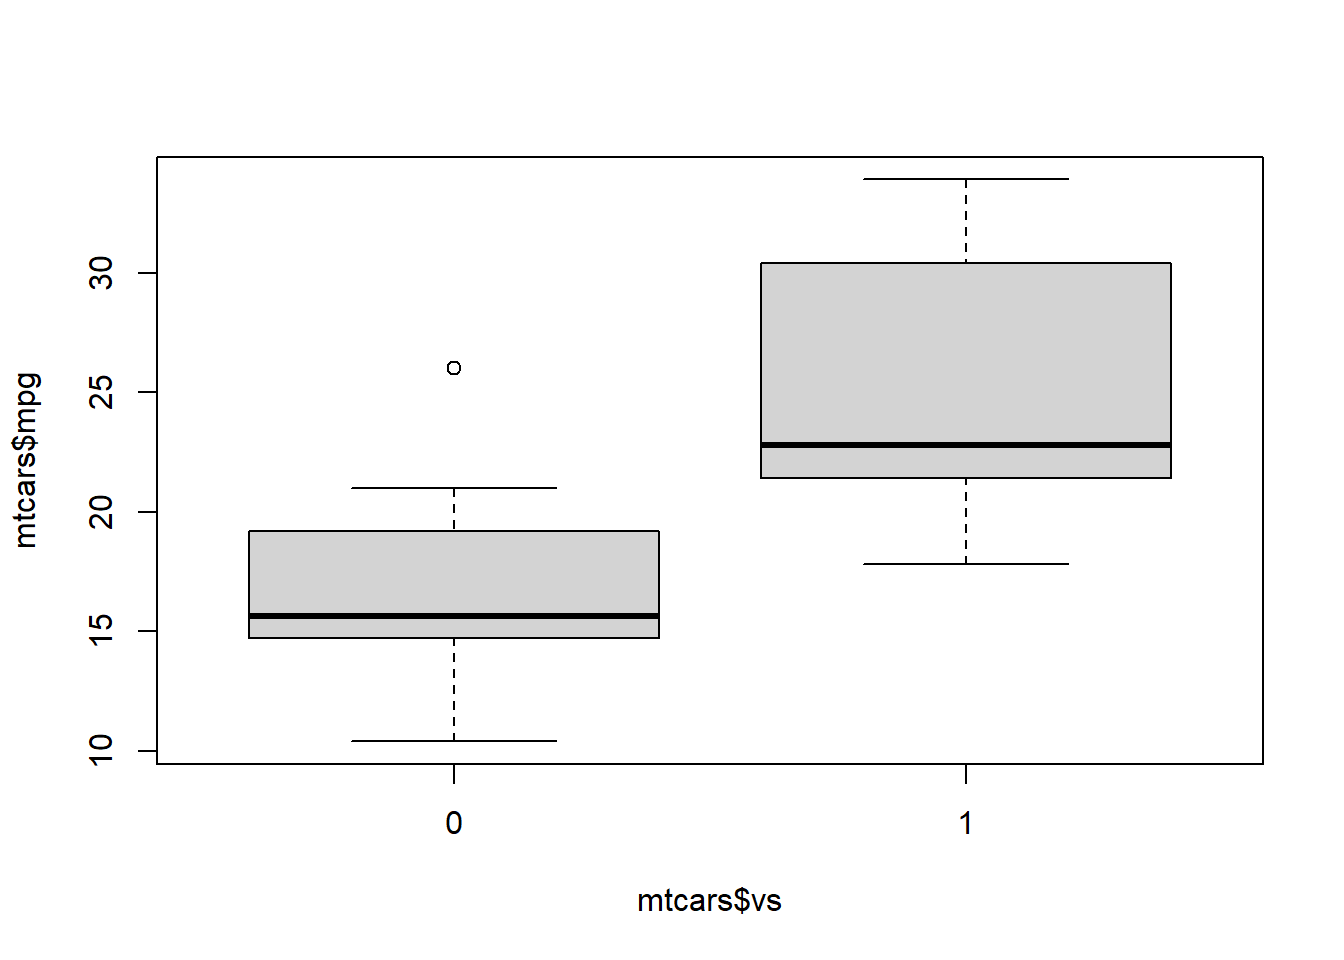
\includegraphics[keepaspectratio]{2.01.-R-base_files/figure-pdf/unnamed-chunk-3-1.pdf}}

\section{boxplot 3}

\pandocbounded{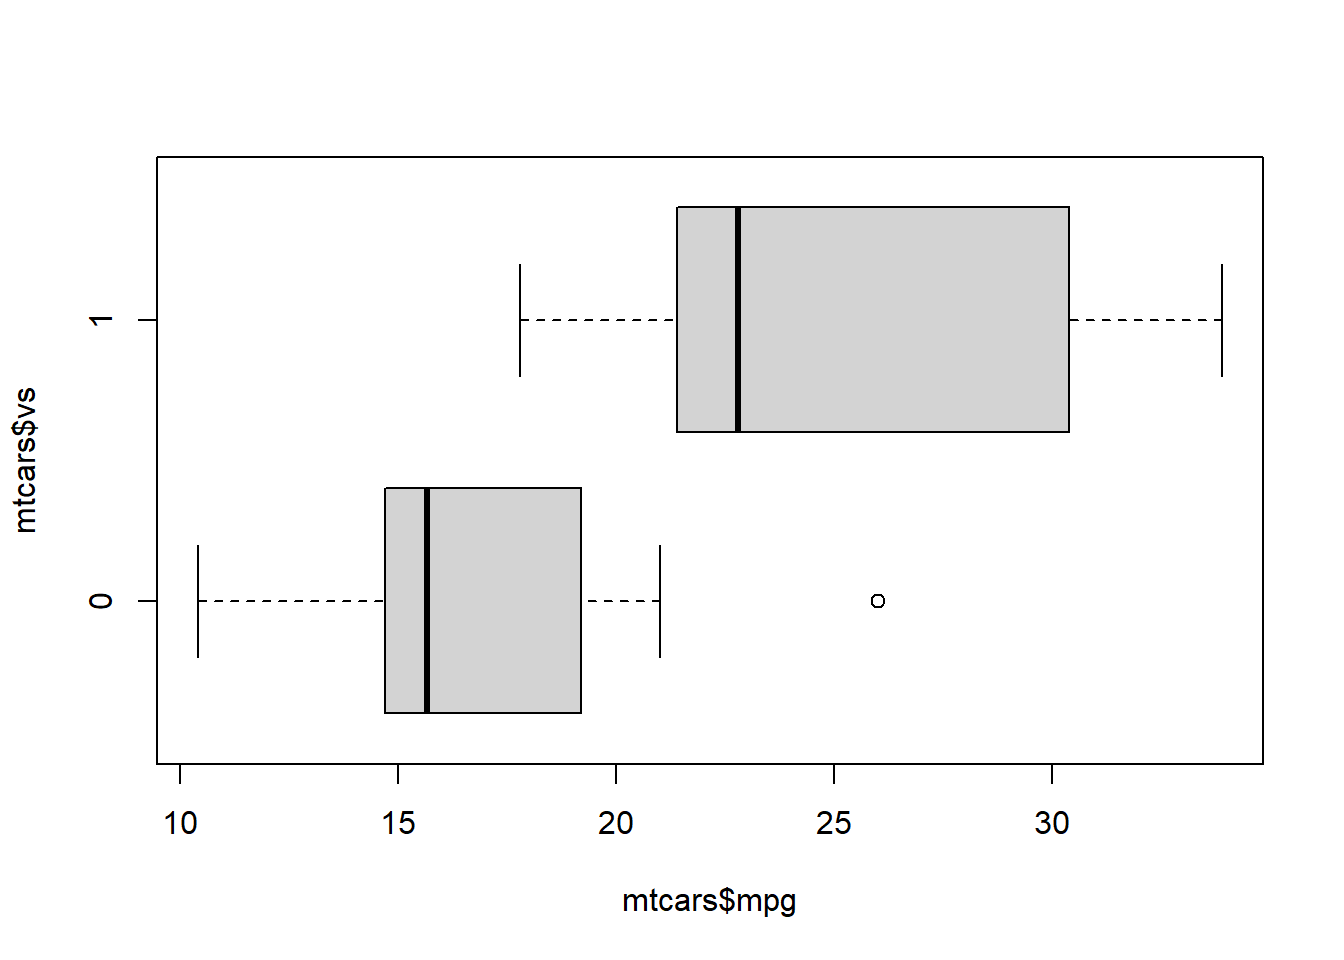
\includegraphics[keepaspectratio]{2.01.-R-base_files/figure-pdf/unnamed-chunk-4-1.pdf}}

\section{Tipos de objetos R}\label{tipos-de-objetos-r}

\section{Pregunta}

\subsubsection{\texorpdfstring{\textbf{¿Qué tipo de variables representa
cada objeto creado en el código
siguiente?}}{¿Qué tipo de variables representa cada objeto creado en el código siguiente?}}\label{quuxe9-tipo-de-variables-representa-cada-objeto-creado-en-el-cuxf3digo-siguiente}

\begin{Shaded}
\begin{Highlighting}[]
\NormalTok{objeto1 }\OtherTok{\textless{}{-}} \StringTok{"Jerry"}
\NormalTok{objeto2 }\OtherTok{\textless{}{-}} \DecValTok{2}
\NormalTok{objeto3 }\OtherTok{\textless{}{-}} \StringTok{"3"}
\NormalTok{objeto4 }\OtherTok{\textless{}{-}} \ConstantTok{TRUE}
\NormalTok{objeto5 }\OtherTok{\textless{}{-}} \FloatTok{1.1}
\NormalTok{objeto6 }\OtherTok{\textless{}{-}} \FunctionTok{c}\NormalTok{(}\DecValTok{5}\NormalTok{, }\DecValTok{4}\NormalTok{, }\DecValTok{3}\NormalTok{)}
\NormalTok{objeto7 }\OtherTok{\textless{}{-}} \FunctionTok{list}\NormalTok{(}\DecValTok{5}\NormalTok{, }\DecValTok{4}\NormalTok{, }\DecValTok{3}\NormalTok{)}
\NormalTok{objeto8 }\OtherTok{\textless{}{-}} \FunctionTok{tibble}\NormalTok{(}\AttributeTok{x =} \FunctionTok{c}\NormalTok{(}\DecValTok{1}\NormalTok{,}\DecValTok{2}\NormalTok{), }\AttributeTok{y =} \FunctionTok{c}\NormalTok{(}\StringTok{"A"}\NormalTok{, }\StringTok{"B"}\NormalTok{))}
\NormalTok{objeto9 }\OtherTok{\textless{}{-}}\NormalTok{ print}
\end{Highlighting}
\end{Shaded}

\section{Respuestas}

\begin{Shaded}
\begin{Highlighting}[]
\NormalTok{objeto1 }\OtherTok{\textless{}{-}} \StringTok{"Jerry"}                              \CommentTok{\# texto (string)}
\NormalTok{objeto2 }\OtherTok{\textless{}{-}} \DecValTok{2}                                    \CommentTok{\# número entero (integer)}
\NormalTok{objeto3 }\OtherTok{\textless{}{-}} \StringTok{"3"}                                  \CommentTok{\# número como texto}
\NormalTok{objeto4 }\OtherTok{\textless{}{-}} \ConstantTok{TRUE}                                 \CommentTok{\# booleano (logical)}
\NormalTok{objeto5 }\OtherTok{\textless{}{-}} \FloatTok{1.1}                                  \CommentTok{\# número decimal (double)}
\NormalTok{objeto6 }\OtherTok{\textless{}{-}} \FunctionTok{c}\NormalTok{(}\DecValTok{5}\NormalTok{, }\DecValTok{4}\NormalTok{, }\DecValTok{3}\NormalTok{)                           }\CommentTok{\# vector con 3 elementos}
\NormalTok{objeto7 }\OtherTok{\textless{}{-}} \FunctionTok{list}\NormalTok{(}\DecValTok{5}\NormalTok{, }\DecValTok{4}\NormalTok{, }\DecValTok{3}\NormalTok{)                        }\CommentTok{\# lista con 3 elementos}
\NormalTok{objeto8 }\OtherTok{\textless{}{-}} \FunctionTok{tibble}\NormalTok{(}\AttributeTok{x =} \FunctionTok{c}\NormalTok{(}\DecValTok{1}\NormalTok{,}\DecValTok{2}\NormalTok{), }\AttributeTok{y =} \FunctionTok{c}\NormalTok{(}\StringTok{"A"}\NormalTok{, }\StringTok{"B"}\NormalTok{))  }\CommentTok{\# base de datos}
\NormalTok{objeto9 }\OtherTok{\textless{}{-}}\NormalTok{ print                                }\CommentTok{\# función}
\end{Highlighting}
\end{Shaded}

\section{Tipos de variables}\label{tipos-de-variables}

\begin{itemize}
\item
  \textbf{String}: texto, siempre se señala con ``\,'' o '\,'.
\item
  \textbf{Numéricas}:

  \begin{itemize}
  \item
    \textbf{Integer}: números entéros.
  \item
    \textbf{Double}: enteros + decimales.
  \end{itemize}
\item
  \textbf{Logical}: valores TRUE o FALSE
\end{itemize}

\section{Operaciones sobre variables}\label{operaciones-sobre-variables}

\chapter{String}

\subsection{Eliminar valores}\label{eliminar-valores}

\begin{Shaded}
\begin{Highlighting}[]
\CommentTok{\#La primera instancia:}
\FunctionTok{str\_remove}\NormalTok{(string, }\StringTok{"o"}\NormalTok{)}
\end{Highlighting}
\end{Shaded}

{[}1{]} ``Hla para UA''

\begin{Shaded}
\begin{Highlighting}[]
\CommentTok{\#Todas las instancias:}
\FunctionTok{str\_remove\_all}\NormalTok{(string, }\StringTok{"a"}\NormalTok{)}
\end{Highlighting}
\end{Shaded}

{[}1{]} ``Hol pr UA''

\subsection{Reemplazar valores}\label{reemplazar-valores}

{[}1{]} ``Holx para UA'' {[}1{]} ``Holx pxrx UA''

\subsection{Separar valores}\label{separar-valores}

{[}{[}1{]}{]} {[}1{]} ``Hola'' ``para'' ``UA''

\chapter{Numericas}

\chapter{Logical}

\section{Loops}\label{loops}

\section{Purrr}\label{purrr}

\part{Módulo UA}

\chapter{Características de la
unidad}\label{caracteruxedsticas-de-la-unidad}

Módulo UA

\hfill\break

\section{TRABAJO EN EQUIPO}\label{trabajo-en-equipo}

La unidad de análisis valora el trabajo en equipo, en concreto se espera
que:

\begin{itemize}
\item
  Se pida ayuda cuando se requiera. En especial si crees que no
  comprendes en su totalidad un análisis o procedimiento.
\item
  Se ofrezca ayuda cuando se esté en condiciones.
\end{itemize}

Otro elemento importante es una actitud flexible y de apertura a hacer
las cosas de forma distinta a la que personalmente creemos es la
correcta. Muchas veces vamos a trabajar con códigos antiguos y/o otras
variables que hagan que tengamos que abandonar la priorización de ``el
mejor código'' y sopesar las distintas variables.

\section{BUEN CÓDIGO}\label{buen-cuxf3digo}

Dicho lo anterior, se valora la creación y ejecución de \textbf{buen
código}, cuyas características son:

\begin{itemize}
\item
  Permiten trabajo inter-conectado con compañeros.
\item
  Es \textbf{trazable}: todo está plasmado en el código, no hay cosas
  hechas ``por fuera``.
\item
  Es \textbf{chequeable}: se puede revisar el paso a paso de forma
  fluida.
\item
  Es \textbf{escalable}: lo que hoy hago para tres cosas, mañana
  funciona fácilmente con 8.
\item
  Es \textbf{reutilizable}: aquello sobre lo que itera puede ser variado
  o cambiado para otros estudioso versiones del mismo estudio.
\end{itemize}

\section{CARACTERÍSTICAS DEL EQUIPO DE
PROGRAMADORES}\label{caracteruxedsticas-del-equipo-de-programadores}

\begin{itemize}
\item
  Tener un lenguaje común.
\item
  Tener perspectiva.
\item
  Documentar adecuadamente el proceso de los procedimientos (uso
  efectivo de comentarios).
\item
  Priorizar diseño por sobre escritura de código.
\end{itemize}

\section{RELACIÓN CON LAS OTRAS
ÁREAS}\label{relaciuxf3n-con-las-otras-uxe1reas}

Típicamente en nuestro que hacer tenemos \textbf{2 principales
relaciones}:

\begin{itemize}
\item
  \textbf{Los clientes internos}: cuando el cliente es de dentro de
  mide.
\item
  \textbf{Los clientes externos}: cuando el cliente es externo a mide.
\end{itemize}

\section{ESTRUCTURA DE CARPETAS}\label{estructura-de-carpetas}

\begin{itemize}
\item
  \textbf{01.} \textbf{Insumos}: todo lo que nos entrega la contraparte.
\item
  \textbf{02.} \textbf{Procedimientos}: donde generamos el código del
  análisis.

  \begin{itemize}
  \item
    Procedimientos \textbf{10}: importación.
  \item
    Procedimientos \textbf{20}: validación y acomodación.
  \item
    Procedimientos \textbf{30}: Análisis.
  \end{itemize}
\item
  \textbf{03.} \textbf{Productos}: resultados y salidas.
\end{itemize}

\bookmarksetup{startatroot}

\chapter*{References}\label{references}
\addcontentsline{toc}{chapter}{References}

\markboth{References}{References}

\phantomsection\label{refs}
\begin{CSLReferences}{1}{0}
\bibitem[\citeproctext]{ref-knuth84}
Knuth, Donald E. 1984. {``Literate Programming.''} \emph{Comput. J.} 27
(2): 97--111. \url{https://doi.org/10.1093/comjnl/27.2.97}.

\bibitem[\citeproctext]{ref-muniz2010teorias}
Muñiz, José. 2010. {``Las Teor{ı́}as de Los Tests: Teor{ı́}a Cl{á}sica y
Teor{ı́}a de Respuesta a Los {ı́}Tems.''} \emph{Papeles Del Psic{ó}logo}
31: 57--66.

\end{CSLReferences}




\end{document}
